\documentclass[letterpaper]{report}
\usepackage{makeidx,verbatim,texhelp,fancyhea,graphicx}
%\input{psbox.tex}
\parskip=10pt
\parindent=0pt
\title{JAZZ++ MIDI sequencer version 5.0}
\author{Donald B. Moore  $<$db.mo@hotmail.com$>$\\
Pete Stieber $<$pstieber@gmail.com$>$}
\date{June 2008}
\makeindex%
\begin{document}
\maketitle%
\pagestyle{fancyplain}
\tableofcontents%

%%%%%%%%%%%%%%%%%%%%%%%%%%%%%%%%%%%%%%%%%%%%%%%%%%%%%%%%%%%%%%%%%%%%%%%%%

\chapter{Introduction}\label{introduction}

JAZZ++ is a fully featured software MIDI sequencer with audio support. In
addition to basic sequencer functions like record and play, JAZZ++ provides
many specialized editing features like quantize, copy, transpose, graphical
pitch editing, multiple undo/redo etc. As an extension to traditional normal
MIDI sequencing, JAZZ++ provides audio play (*.wav files), audio recording and
audio/midi integration. A multi function {\em audio editor} is also included.

JAZZ++ has support for {\em GM} (General MIDI) equipment with both {\em GS}
and {\em XG} extensions, and also offers special functions like GS/XG sound
editing, setting of effect types, a {\em random rhythm generator} and a {\em
harmony browser}. Windows versions of JAZZ++ can be synchronized to other sound
equipment (e.g. a tape recorder) using MIDI Time Code (MTC) or SongPointer
synchronization techniques. [ed: is this still only so for the Win version??]

JAZZ++ is a platform/OS independant software program, and has been designed to
work on Windows and Linux operating systems using 32bit or 64bit Intel ix86
based computers (the 'PC'), and also for MacOSX using Mac computer systems. [ed:
ppc? intelmac? m680x0? ;-] Being a MIDI based program, JAZZ++ can interact with
both externally connected MIDI equipment (MIDI capable keyboards, synthesizer
modules, drum-machines etc), internally connected MIDI equipment (soundcards
with hardware based MIDI/synth capabilities), or with one or more MIDI capable
software synthesizer programs ('softsynths') running on the same computer as
JAZZ++. [ed: I'd like to add something here...is it possible ...or going to
be...to use combinations of all of these?]
 


[ed:..actually, this belongs in it's own chapter above trackwindow, with a
title like 'Overview of working with jazz++'...then this bit below would
fit.....]


JAZZ++ has two main windows; one
operating on the song as a whole, and one operating on single tracks and
single events. Among the other windows and dialogs are mixer windows for easy
adjusting of default track parameters, and all settings are saved into the
MIDI file for later use.


[ed:...and carry on with some bits removed from track/piano/audio chapters
 below which are more to do with basic -program- operations and nothing
to do with -tracks- (or the editing thereof) at all for instance.] 

%%%%%%%%%%%%%%%%%%%%%%%%%%%%%%%%%%%%%%%%%%%%%%%%%%%%%%%%%%%%%%%%%%%%%%%%%
\section{System requirements}\label{requirements}

JAZZ++ is a software MIDI sequencer that makes it possible for the JAZZ++
user to employ everyday personal computing hardwares, and other connected MIDI
based equipment, to potentially create a very powerful and highly featured
Digital Audio Workstation (DAW). The performance of JAZZ++ itself when used
is this manner, is primarily dependent on just how capable/powerful the user's
computer system actually is  This section briefly describes the various minimum
hardware and software requirements needed for satisfactory operation using the
JAZZ++ software MIDI sequencer.

The original Jazz++ documentation recorded here;

"To play MIDI music your PC must be attached to a MIDI synthesizer device. The
synthesizer can either be an integrated part of a sound-card, or an external
device attached to the PC with a cable. To record MIDI music you will need a
midi-capable piano-keyboard attached to the PC (as an alternative you can enter
notes using the mouse). For audio you need an audio capable sound card."

It is now 2008, and a lot has changed in the computing hardware and software
arenas since the original JAZZ++ documentation was drafted some time around
1995. While the above paragraph is more or less still correct, it was written in
a time before modern computers had 'onboard' sound hardware like most people
have now-a-days. Likewise, back in those days software based MIDI synthesizers
were not as functional (nor as plentiful) as they are today, so you really
\underline{don't} need any 'real' MIDI hardware to play MIDI music on your PC
anymore -- you can use a software synthesizer (softsynth) instead.


\subsection{Operating Systems supported by JAZZ++}

The current version of JAZZ++ is known to work with the Windows, Linux, and
MacOSX operating systems. You will need to be running one of these operating
systems on your computer hardware to use JAZZ++.

\subsection{Computer Architectures supported by JAZZ++}

The current version of JAZZ++ is known to work with most all computer
architectures supported by the above Operating Systems. This includes the
Intel based 'PC' hardware platforms (x86\_32bit and x86\_64bit), and also Mac
computer system hardwares.[ed: bit more clarity with the Mac stuff here]

\subsection{Software pre-requisites of JAZZ++}

The current version of JAZZ++ uses the wxWidgets GUI library to create
the JAZZ++ user interface. The wxWidgets GUI library, like JAZZ++ itself,
is platform/OS independant, and versions of wxWidgets are available for
all platforms/OS' currently supported by JAZZ++. If you do not have the
wxWidgets GUI library installed, please visit the following link to download
and install wxWidgets for your platform/OS ;

\begin{indented}{2cm}
\htmlonly{\urlref{http://www.wxwidgets.org/}{http://www.wxwidgets.org/}}
\latexonly{http://www.wxwidgets.org/}
\end{indented}

The wxWidgets GUI library \underline{must be installed} before installing
JAZZ++ itself.


\subsection{Recommended Computer Specifications for using JAZZ++}

How powerful your computer system needs to be, is determined primarily by
how you use it with JAZZ++ ....ie; if you are going to be using JAZZ++ on
a computer system that is also running a MIDI 'softsynth' for the actual sound 
rendering and reproduction, you will need more computing power compared to 
using JAZZ++ with the same computing hardware and having MIDI/synth soundcards
and/or external MIDI devices connected to it instead.

Generally speaking though, any 'modern' computer system (post-2000) with a
1GHz or greater CPU speed and 512Mb or system ram, should easily run JAZZ++
in normal use. Even computer systems older than this date might be perfectly
capable or running JAZZ++ depending on what you are doing and how much system
ram that older computer has. More details of the actual requirements needed here
are discussed in the 'Installation and Setup' chapter of this manual, and
various platform/OS specific informations can be found in this manual's
Appendix section. 

\subsection{MIDI devices supported by JAZZ++}

JAZZ++ supports all standard MIDI protocols and commands, and as such should
work with any standard MIDI capable equipment and/or musical instruments. JAZZ++
also supports most 'virtual' MIDI devices, such as software synthesizers, other
software MIDI sequencers and trackers, and software virtual MIDI keyboards - if
it's MIDI, it should work with JAZZ++ 'out of the box'.


\section{Where to get it}\label{wheretoget}

For the latest JAZZ++ updates from {\em sourceforge}, please look at the JAZZ++
homepage at ;

\begin{indented}{2cm}
\htmlonly{\urlref{http://jazzplusplus.sourceforge.net}{http://jazzplusplus.sourceforge.net}}
\latexonly{http://jazzplusplus.sourceforge.net}
\end{indented}

[ed: make the above link point to downloads page? ]

If you are interested in developing JAZZ++ or want to check out the latest
'bleeding edge' version of the JAZZ++ source code, you can always checkout the
JAZZ++ Subversion repository at ;

\begin{indented}{2cm}
\htmlonly{\urlref{http://jazzplusplus.sourceforge.net/subversion}{http://jazzplusplus.sourceforge.net/subversion}}
\latexonly{http://jazzplusplus.sourceforge.net/subversion}
\end{indented}

\section{Getting Help with JAZZ++}

You are welcome to join the JAZZ++ mailing lists if you require any additional
or specific help with JAZZ+ usage and setup not covered by this manual. The
JAZZ++ mailing lists give JAZZ++ users the facility to discuss problems they
might be having with JAZZ++, with both other users of the software -and- the
developers of JAZZ++ itself.

The JAZZ++ developers are a faily easy going bunch of people, and they really do
look forward from hearing from you, however, to protect both themselves and
other subscribers to the JAZZ++ mailing lists from 'SPAM', they ask that people
who join and post emails to the JAZZ++ mailing lists adhere to the following
two points of list etiquette ;

'PCYMTNQREAIYR'

\underline{Please Configure Your Mailer To Not Quote Raw E-mail Addresses In
Your Replies.}
Some email programs ('Mailers') by default include the raw e-mail address in the
"Joe <joe@example.com> wrote:" line. The web archives for the mailing lists are
publicly available. Let's not feed the spam harvesters! Mailing lists are
routine targets for spam software to come looking for valid email addresses, and
if you include raw email addresses in your email replies you may well be
inadvertantly and innocently unaware that you're actually helping such spam
operations in doing so. People who use their web-browser and one or another of
the free public email servers available... like hotmail, yahoo and so on...have
to be particularly careful with this, and you may find that you have to manually
delete raw email addresses from you replies to comply with this etiquette.

'PCYMTWLL'

\underline{Please Configure Your Mailer To Wrap Long Lines.} Some email programs
don't, and
this is especially so when a web-browser interface is being used, and then most
of the message ends up looking like one lo-ong line in the web archives. It's
very annoying to have to scroll left and right as well as up and down. Please be
considerate of this situation! All you have to do is remember to hit the return
[enter] key at about 80 characters along each line, and start a new line. Your
email text in an web-browser window, should appear as a column in the left of
your web-browser window, not as a document that fills the entire window page. It
makes it easier for everyone if you please comply with this etiquette when
submitting emails to the lists. 

\begin{indented}{2cm}
\htmlonly{\urlref{http://jazzplusplus.sourceforge.net/mailinglist}{http://jazzplusplus.sourceforge.net/mailinglist}}
\latexonly{http://jazzplusplus.sourceforge.net/mailinglist}
\end{indented}


There are three mailing lists.  The first is a devoted to JAZZ++ users.  To
subscribe, please visit ;

 [ed: double check these links below]

\begin{indented}{2cm}
\htmlonly{\urlref{https://lists.sourceforge.net/lists/listinfo/jazzplusplus-user}{https://lists.sourceforge.net/lists/listinfo/jazzplusplus-user}}
\latexonly{https://lists.sourceforge.net/lists/listinfo/jazzplusplus-user}
\end{indented}

The second is devoted to developers.  To subscribe visit

\begin{indented}{2cm}
\htmlonly{\urlref{https://lists.sourceforge.net/lists/listinfo/jazzplusplus-devel}{https://lists.sourceforge.net/lists/listinfo/jazzplusplus-devel}}
\latexonly{https://lists.sourceforge.net/lists/listinfo/jazzplusplus-devel}
\end{indented}

The third list contains messages generated by developers when they commit
documentation, web content, or code to the JAZZ++ subversion repository.
To subscribe visit

\begin{indented}{2cm}
\htmlonly{\urlref{https://lists.sourceforge.net/lists/listinfo/jazzplusplus-updates}{https://lists.sourceforge.net/lists/listinfo/jazzplusplus-updates}}
\latexonly{https://lists.sourceforge.net/lists/listinfo/jazzplusplus-updates}
\end{indented}

We'd also be happy to receive your bug reports (well, somehow). We want to find
and fix any problems with JAZZ++, so bug reports are welcomed. Before you do
send any email regarding a possible JAZZ++ bug, please be sure to read the
JAZZ++ Reporting Bugs page on the JAZZ++ website, for instructions on how
to gather the necessary informations JAZZ++ developers might need to fix the
problem, and how to submit that bug report in a meaningful and consistant way ;

\begin{indented}{2cm}
\htmlonly{\urlref{http://jazzplusplus.sourceforge.net/bugreports}{http://jazzplusplus.sourceforge.net/bugreports}}
\latexonly{http://jazzplusplus.sourceforge.net/bugreports}
\end{indented} 


//...this subpara below should be melded into the above somewhere...//
[ed: probably to get it to hit -user instead of -devel..fix l8r]

 or success stories. And - of course - you are welcome to contribute to the
JAZZ++ project by sending code, suggestions, ..., or corrections for this
manual.

\section{Acknowledgments}

JAZZ++ is based on the work of countless other people who have have made
their software freely available. Beside all the people who made Linux,
GNU and X11 possible, we'd like to mention

\begin{itemize}
\item {\em Hannu Savolainen} for writing all these excellent midi drivers, so
JAZZ++ can talk to nearly every midi card on Linux.
\item {\em Julian Smart} who wrote the free, portable GUI library
wxwin, so JAZZ++ runs with XView, Motif and MS-Windows.
\end{itemize}

We would also like to thank Henrik Seidel and Stefan Nitschke for code
contributions.

[ed: is the above complete for this section?]

\section{Copyright}\label{copyright}

The JAZZ++ MIDI Sequencer is copyright (C) 1994-2000 Andreas Voss and
Per Sigmond, all rights reserved.

[ed: Pete's name should be here somewhere too ]

JAZZ++ program is free software; you can redistribute it and/or modify
it under the terms of the GNU General Public License as published by
the Free Software Foundation; either version 2 of the License, or
(at your option) any later version.

This program is distributed in the hope that it will be useful,
but WITHOUT ANY WARRANTY; without even the implied warranty of
MERCHANTABILITY or FITNESS FOR A PARTICULAR PURPOSE.  See the
GNU General Public License for more details.

You should have received a copy of the GNU General Public License
along with this program; if not, write to the Free Software
Foundation, Inc., 675 Mass Ave, Cambridge, MA 02139, USA.

%%%%%%%%%%%%%%%%%%%%%%%%%%%%%%%%%%%%%%%%%%%%%%%%%%%%%%%%%%%%%%%%%%%%%%%%%%%%%%%%

\chapter{Installation and Setup}\label{installation}

This chapter of the JAZZ++ manual, describes how to install JAZZ++ itself
on the three platforms/OS' currently supported, and how to setup the MIDI
and computer hardware systems for use with JAZZ++. Although most all the
various features and functions of JAZZ++ work identically for all supported
OS types and computer platforms, there are small inherent differences on
how to do things relative to which platform/OS you might be using when it 
comes to installing and setting up the systems for use with JAZZ++ itself.

If you are new to JAZZ++ and the MIDI domain, you are encouraged to read the 
following sections to gain some insight about how things work, and how they
fit together to complete the final system setup for use in conjunction with
the JAZZ++ software MIDI sequencer.

On the other hand, if you're already conversant with MIDI operations and just
want to get on with the installation and setup process, feel free to skip the
following descriptive passages and move on to the OS specific instructions
that appear later in this chapter. 


\section{MIDI and audio equipment}

The term 'MIDI' is an acronym - it stands for (the) 'Musical Instrument Digital
Interface'. It is an industry-standard protocol that enables electronic musical
instruments, computers, and other MIDI capable equipment to communicate,
control, and synchronize with each other using a common 'language'. The MIDI
protocol does not deal with audio data itself, but instead transmits (and
receives) MIDI data that..for example...tells the connected MIDI synthesizer
what note to play, when to play it, and how to play it. In recent years with
the many advances in both electronics and computer technologies, it has been
possible to incorporate both MIDI functionality and audio editting facilities
into the same MIDI domain, and both dedicated MIDI hardware equipment, and 
software based MIDI programs like JAZZ++, have audio (sound file) manipulation
facilities builtin.

Back when the original Jazz++ was being developed, there weren't many 'software
synthesizer' programs available for the personal computer, and even if they were
available, the then computing hardware was simply too slow to run such software
properly. A lot has changed since then and now. Today, even so called 'entry
level' personal computers have more than enough power to run Jazz++ concurrently
with one (or more) 'software synthesizers' running on the same machine, thus
making it possible for Jazz++ to become the basis of a fully functional Digital
Audio Workstation (DAW) using otherwise standard, low cost personal computer
systems and/or other now affordable add-on sound/MIDI hardware options.


If you're not using a hardware MIDI/synth soundcard or externally connected
MIDI synthesizer, you will need an audio capable soundcard to hear anything.
Today however, most personal computers already have 'onboard' audio sound
chipsets, so for most people it's very likely that you already have this
requirement satisfied. Likewise, MIDI/synth capable addon soundcards are a -lot-
cheaper today than when Jazz++ first started out, and you can buy MIDI/synth
soundcards of various types for under 50 dollars these days. One can also buy
high-end MIDI/synth soundcards for a few hundred dollars if you're looking for
the very best quality sound ouput, or many otherwise 'professional' features 
and specifications such soundcards boast.

If on the other hand you do intend to use JAZZ++ with one or another external
MIDI devices/instruments connected to your computer, you will need to install
and setup your OS dependant drivers to be able to communicate with whatever
computer-to-MIDI interface and equipment you happen to be using. It is common
practise today to use the USB computer port to connect such hardware MIDI
interfaces, however there are examples that use the serial port, the parallel
port, or otherwise come as an addon computer interface card instead. Whatever
hardware is used, the OS specific drivers must be installed and configured for
use with JAZZ++. Unfortunately, it is beyond the scope of this manual to give
JAZZ++ users any specific help with this task, if for no other reason than the
JAZZ++ team simply not having hands-on access to every possible MIDI interface
type in the world today. This is further recited, in the OS specific sections
of the manual appearing in this chapter.
 

This area of the Jazz++ documentation provides information explaining common
concepts of working with MIDI and the personal computer, and details how to
get the most out of you personal computer when using it with Jazz++, and also
platform/OS specific information regarding setting up and using Jazz++ with the
now available computer hardware technologies and various 'software synthesizer'
MIDI programs available to the personal computer user today.


\section{Common Considerations when using Jazz++}

\subsection{CPU and RAM Requirements}

CPU

The original Jazz++ user manual advised -- "For MIDI-only operation
a 486 CPU (or equivalent) is sufficient in most cases.  For satisfactory audio
operation a Pentium CPU with 32 MBytes RAM is recommended." That may well be
true for MIDI only operations with no sound of any kind being needed to be
produced by the computer hardware. Perhaps we will never know for sure how well
Jazz++ ran on such computing powerhouses as the i486 CPU running at a then
whopping 100MHz, because most of this hardware is now dead and gone.

Most modern personal computer systems now boast CPU speeds in excess of 1.5 GHz
-- even a new low-end 'entry level' computer system is likely to be running at
speeds greater than 2.0GHz. This should be more than enough computing (CPU)
power to run and use Jazz++ effectively on a modern personal computing machine,
even with softsynths running to produce the actual sound itself.

RAM

As mentioned earlier, Jazz++ itself should not present any significant system
load to the personal computer it's being run on. Likewise, Jazz++ doesn't need a
lot of system RAM to work correctly with modern computer hardwares. The user
will however need enough system RAM installed to meet the following requirements
for smooth and trouble free Jazz++ sessions ;

1. You will need enough system RAM installed to cover your computer's system
requirements without the system needing to access the hard-disk based 'swap' (or
'pagefile') area of RAM whilst using Jazz++. Compared to real 'chip' RAM,
hard-disk based RAM devices are incredibly slow and this can 'bottleneck'
other system operations. More importantly, to access hard-disk based RAM means
generating a lot of hardware interrupts at the same time. Doing this is very
likely to impact on MIDI playback and record operations in Jazz++ and introduce
timing latency issues.

2. If you use soundfonts with MIDI/synth soundcards or softsynths (and you
probably will do), you need enough system RAM to hold these soundfile libraries,
-above- the system RAM requirements. Soundfont libraries are loaded into RAM,
and whilst a lot of soundfont files are small (<1mb), others can be quite large
(100+mb), and depending on how many soundfont libraries you intend to use and
how big they are, dictates exactly how much RAM you will need here.

It is nearly impossible to correctly and accurately predict just how much CPU
speed and system RAM is needed in every individual's case -- there are just too
many variables to consider. To give the reader some idea though, the following
are results observed by one of the Jazz++ testing team ;

[ed: add system stats]



*NEW*

\subsection{MIDI, Time and the Personal Computer}

The MIDI protocol attempts to be a real time protocol. This is unsurprising --
sound generation and replay (of a song or most all musical compositions) happens
in real time, the audience and/or the recording studio hear the performance in
real time. If you are a performer on stage using MIDI equipment, that MIDI
equipment must be operating as close to real time performance as it possibly can
-- when the performer plays a note on a MIDI keyboard, that note event should be
heard almost instantaneously not in 5 to 200 milliseconds of time after the
event. Likewise, every note event should be acted upon - if the MIDI track is
sequenced to produce 8 beats on a kick drum voice, you should hear the
synthesizer produce 8 beats of that voice, not 7 beats.

Time (with regards to MIDI) is what we used to measure the actual deviation from
'real' time that the MIDI response time effectively is. Remember, I stated MIDI
*attempts* to be a real time protocol, but in actual practice it very rarely is.
There are latencies in various parts of the MIDI chain -- even the physical
length of the MIDI patch-cords introduce latency..albeit small..into the
interconnected MIDI device chain. The response time of the MIDI instrument
receiving a transmitted note event is another place latency can be experienced,
and if you are using Jazz++ to trigger another externally connected MIDI device
which itself is a sequencer, the timing is even more important to help ensure
everything starts, plays, and remains 'in sync'.

The above two paragraphs are things common to the MIDI domain that MIDI users
have always had to deal with, regardless of whether or not a PC was being used
in the MIDI chain. As a matter of fact, a 'virtual' MIDI chain involving
softsynths and Jazz++ running on a PC, is subject to exactly the same kinds of
limitations and latency problems as 'real' MIDI equipment does...plus one extra
layer -- the inherent amount of latency in the operating system and PC hardware
being used to 'host' the virtual MIDI machines and software programs.

When using a PC in this fashion, there are possible latencies in a few different
places of the setup overall ; how fast the 'host' system executes (runs) Jazz++
itself, how fast the generated note events can be delivered to/from the
computer's hardware ports, and/or how fast these same note events can be
delivered to and be rendered by a softsynth running concurrently on the same
system. Just how powerful your particular hardware is does matter, however there
are some common methods and practices that can be employed to better tailor how
your personal computer performs with Jazz++. There are also some platform/OS
specific 'tweaks' that can be employed to help make your platform of choice run
better when using Jazz++ with timing critical protocols such as MIDI on the
modern day PC.

Running Jazz++ should not impose any significant system load by itself, however
it does rely on the operating system to deliver the MIDI data to the intended
hardware/virtual ports, and also for delivering software data to the computer's
graphics adapter for GUI updates..ie; track window scrolling.

No matter what PC hardware you are using, most all of this software data has to
be processed by (or pass through) the operating system in use, and most modern
operating systems allow the software programmers to use so called 'real time'
kernel calls, and direct, immediate access to I/O ports and so forth to the
actual computer hardware itself. On some platform/OS types this doesn't happen
automatically, and some users might have change some system configurations to
achieve optimum performance when using Jazz++ and MIDI on their personal
computing machine.

\subsection{SoundFonts - what are they, who needs them.}

Soundfonts are data files that both hardware MIDI/synth cards and MIDI
softsynths may use to create (or synthesize) the actual sound you hear playing.
Soundfont files, typically end in the .sf2 .SF2 extensions, although you may
also find .sfArk or .sfpack files, which are normal .sf2 packages compressed
with a lossless encoding tool. A multitude of free soundfont packages exist on
the internet, most of them quite good however some have decidedly better sound
quality than others. There are also soundfont editors available for most
platforms supported by Jazz++, which allows the user to create their own custom
soundfont library file.

A soundfont itself is a software library file containing both sampled audio
data, and synthesizer parameter definitions, along with the table of MIDI data
that describes the 'soundbank' itself. The soundbank presents itself to the
user, as a list describing exactly what instruments, voices, or sounds are
contained in each soundfont library file. Taking your time to search for 'the
right' soundfont for your use can take a bit of trial and error, but it's well
worth the trouble. On the other hand, you can also buy high quality soundfont
libraries from commercial companies, if one needs first quality performance.

Many MIDI/synth soundcards require soundfont files to work, and the softsynth
setup described further on in this manual also requires 1 (or more) soundfont
files to actually make any pleasing sounds. Although the FLUIDSYNTH package
includes it's own sample soundfont file, the quality is not the best...which
you'll discover, when you download and install your own soundfont files. In the
Appendix section of the manual, is a short list of soundfont resources we here
at Jazz++ think you should try. 


\subsection{Jazz++ operational tricks}

1. Try lowering your desktop resolution and/or bits-per-pixel value. Doing this
will also lower the load on your CPU when running Jazz++, and enable things to
run closer to real time overall. Try using the lowest possible resolution and
screen dimension that you can -comfortably- work with while using Jazz++ at a
color depth of 8 bits-per-pixel, and see if that helps real time performance.

2. The ZOOM buttons are your friends! To avoid unnecessary system load when
running record/replay sessions with Jazz++, always remember to zoom out so the
track window graphics are in complete view with no need to paginate the window
scrolling operation. Zoom in again if you want to edit a portion of a track.
Having to paginate and scroll the Jazz++ track window, generates hardware
interrupts which may impact real time performance.

3. Try to have as few software programs running in the background at the same
when using Jazz++ on a computer system. Really serious Jazz++ users will try to
have the absolute minimum of other software programs running when using Jazz++,
to ensure they get as close to real time performance as is possible using Jazz++
on their personal computer.

4. If you are using other MIDI softwares or MIDI softsynths in conjunction with
JAZZ++, if possible (and where applicable), use the relevant user GUI interface
to set these 'virtual' MIDI entities up, but when actually playing or recording
MIDI compositions, launch these programs from the commandline instead. Use the
'--quiet' commandline switch if it's available. Having to render the GUI
interfaces for such MIDI programs...especially when that GUI contains elements
such as blinking transport running lights or 'RT' (real time) meters...steals
valuable CPU cycles JAZZ++ (or any softsynth) might have otherwise used for it's
own operations.


 
\section{Windows operating systems}

For Windows there is an install utility (run {\tt setup.exe}) which
mostly automates the installation process.

JAZZ++ supports the windows MIDI / audio driver interface. A driver for your
MIDI interface card or sound card must be installed before JAZZ++ can play /
record MIDI or audio.

Provided such a MIDI driver is installed in your system, JAZZ++ currently
supports 32-bit platforms.

\section{Linux operating systems}

For Linux there is a shell script {\tt install-jazz} in the
distribution. You must be logged in as root when running the installation
script. As a default JAZZ++ will be installed to {\tt /usr/local/jazz},
this may be changed by editing {\tt install-jazz}. Also you
must set the environment variable JAZZ to point the jazz directory by
adding the line:

{\tt export JAZZ=/usr/local/home}

to your .profile or .bashrc. Please refer to the file
{\tt install.txt} which contains up-to-date instructions.

On startup JAZZ++ looks for its configuration files
\begin{enumerate}
\item in the current directory
\item in the home directory (where the environment variable HOME points to)
\item in the directory where the environment variable JAZZ points to
\item in the directory from where JAZZ++ itself was started.
\end{enumerate}
The main configuration file is named {\tt jazz.cfg}.
This file also contains pointers to other configuration files {\tt (*.jzi)}
present in the same directory.
Then JAZZ++ searches for a song named {\tt jazz.mid} in the current directory
and loads it - if found. This song may contain default settings for your
midi equipment.


[ed: This part, down to my out mark, should probably go]

The device-independent part of JAZZ++ (the sequencer / editor part) is known
to run on Linux, Sun-OS4 and Solaris2 systems, but should compile and run
(with some minor hacking) on any system supporting Linux/X11. To compile you
will need the wxWidgets GUI package together with GTK.

The device-dependent part (midi-driver) currently supports:

\begin{enumerate}
\item OSS/Free (OSS/Linux) midi driver API (formerly known as USS/Lite and
VoxWare). This API is included in later Linux kernels. The JAZZ++ code
interfacing OSS has only been tested on Linux platforms.
\item JAZZ++'s native MPU-401 midi driver (requires an intelligent-mode MPU-401
interface-card). The driver is implemented as a Linux kernel
load-module. In this mode JAZZ++ works as a TCP/IP-based client/server
application allowing the sequencer/editor and the midi-driver to run on
separate computers. The native driver has better support for the MPU-401
than the JAZZ++/OSS solution (e.g. support for external timing source).
\end{enumerate}

[ed: and be replaced with something more current...ie; if it still
works on Sun-OS4 and Solaris2 systems currently is unknown, USS/lite
and voxware..?..and I thought mpu-401 was dinosaured? I'll get some
clarity before I deal with the section above. *MARK* ]

\begin{itemize}

\item *New*

\end{itemize}


Introduction

Years ago when the Jazz++ project first came to my attention,
using it with Linux on the PC was a much different proposition to
what is possible today on this platform/OS. Although it would be
entirely possible to create a MIDI score with jazz, (in the same way
this text is being produced with a text-editor), the whole point of
the exercise would be to compose a MIDI score you could actually hear.

Back then with Linux, making sound via MIDI applications meant having
MIDI *hardware*. This may have taken the form of a MIDI adapter plugged
in the PC's serial port or soundcard gameport (in MPU-401 mode), with a real
world MIDI instrument(s) attached to that, or else a MIDI capable soundcard
with a hardware based MIDI sound synthesis chip to make the actual sound.
(so called 'MIDI/synth' capable soundcards) In that latter case, the
soundcard necessarily had to be supported by Linux drivers, and in that
respect these drivers were more than likely using the now deprecated 'OSS'
sound system modules.

Things have changed. The x86 based hardwares have become faster and
cheaper, Linux has grown and matured as an operating system, and
likewise Free software has multiplied and proliferated around the world
giving rise to the creation of a great many new software applications.
Along the way, the venerable 'OSS' sound system drivers were replaced
with the 'Advanced Linux Sound Architecture' (ALSA) drivers and API.

The result of these many advances and changes over time, means Linux
users are no longer constrained by the need of having actual MIDI
capable hardware or a MIDI/synth capable soundcard, to obtain good sound
production with MIDI applications like Jazz++. Instead of having one
or more hardware sound synthesis chips (be they on a soundcard or
in a MIDI musical instrument) to produce the sound(s), we can now
use a software application to achieve the same ends, and many folks
loosely refer to these software applications as being 'softsynths'.

For many years now, users with Windows on their PC have had a distinct
advantage over Linux users on the PC, because virtually every sound
card (and/or 'onboard' sound chip) typically ships with proprietary
Windows drivers that enable the use of that hardware as a 'softsynth' in
conjunction with the underlying Windows sound API supports. In effect,
Windows users could come to the website, download Jazz++ and install it,
and be making noise in under 2 minutes with very little or no effort. If
only users of other platforms/OS' could have it this easy - hopefully
this documentation will help bridge the gap, when using Jazz++ on this
platform with MIDI softsynth implementations.



\subsection{Command line options (Unix only)}

Command line options (in any order):

\begin{itemize}
\item {\tt jazz -h}                                   -- Print help text
\item {\tt jazz -v}                                   -- Print help text
\item {\tt jazz -f filename}                          -- Input midi file
\item {\tt jazz -trackwin xpos ypos [width height]}   -- Position/size of main
window
\item {\tt jazz -pianowin xpos ypos [width height]}   -- Position/size of piano
roll window
\end{itemize}


\subsection{Hardware based sound synthesis and Linux on the x86 PC}

Thanks to all the great work done by the ALSA team over the years, Linux
now has much better driver supports for the various soundcards on the market
today that have hardware based MIDI/synth chips as part of their design.

One of the main benefits of using MIDI/synth based soundcards (and
this is true for all platforms), is that it removes the system overhead
of having a softsynth running -- the MIDI data output of Jazz++ is sent
directly to the hardware MIDI/synth chip on the soundcard, and it takes
care of generating the actual sound (and sound data) itself. This allows
the kernel to be closer to 'real time' when using Jazz++, because the
system CPU isn't having to 'play' the sound, and render that sound, all
at the same time. A good analogy, would be to compare all this to the
difference it makes to system -graphics- performance, when you add
a dedicated 3D graphics-card with it's own onboard processor unit. Not
only are the graphics greatly improved, the system responsiveness is
greatly improved as well.

Adding a dedicated MIDI/synth soundcard to your system helps for
exactly the same reasons here - it frees up your system CPU so it
can do other tasks. In Linux, drivers for more than a few of these types of
MIDI/synth soundcards are already available, and are a standard part
of the Linux kernel tree. Most Linux distributions include so called
'hardware detection' softwares, which should automatically discover
your MIDI/synth soundcard (if supported), and configure your system's
ALSA drivers accordingly. Sometimes these routines do not detect certain
hardware cards correctly (or at all) in some situations, however it is
beyond the scope of the Jazz++ manual to help people with problems of this
nature.

The correct place to get help with specific ALSA / soundcard related
problems, can be found by visiting the ALSA website at ;

\htmlonly{\urlref{http://www.alsa-project.org/}{http://www.alsa-project.org/}}
\latexonly{http://www.alsa-project.org/}

The latest list of ALSA supported MIDI/synth soundcards, is always
available inside the current alsa-driver source tarball available from
the above website. Once you unpack that archive, read the file ;

alsa-driver-1.0.1x/doc/SOUNDCARDS

There you can see if your MIDI/synth soundcard is currently supported
under ALSA and Linux. Some MIDI/synth soundcards require firmware being
loaded before the card will work - most all of these kinds of soundcards
require some kind of helper application called a 'loader' to copy various
instrument files and data (for example 'soundfont' files) into the working
RAM of the MIDI/synth chip. Documentation regarding these things and help
with configuring ALSA itself can be found in the same alsa-driver archive ;

alsa-driver-1.0.1x/alsa-kernel/Documentation/


Another good repository of current knowledge regarding Linux sound drivers
overall (not just the ALSA sound drivers) can be found at ;

\htmlonly{\urlref{http://linux-sound.org/drivers.html}{http://linux-sound.org/drivers.html}}
\latexonly{http://linux-sound.org/drivers.html}

Once you have your MIDI/synth soundcard up and running, it will appear
in Jazz++ configuration dialogs just like any other MIDI device connected
to the computer running Jazz++. Using a hardware based MIDI/synth soundcard,
is very much like using a software based 'softsynth' as described below -
you still have to decide which soundfonts to use, and which bank to load them
into. Hardware or software, they are both MIDI instruments, and share very
common ways of getting things done at this level.




\subsection{Software based sound synthesis and Linux on the x86 PC}

This area of the documentation will grow over time. There is a lot
that can be documented here now with Linux.

In the early stages of the current Jazz++'s revitalization, developers,
users and testers alike of the Jazz++ source code used softsynths. One
of the softsynth setups used by the Jazz++ developers and testers in Linux,
is as I describe below, which uses JACK, FLUIDSYNTH and QSYNTH. A similar
setup should also work on the Mac running Mac OSX.

Essentially, -any- ALSA based, MIDI capable softsynth setup should work
with Jazz++ in Linux. I've already tested a few that seem to work fine.
However, it is useful to know how to setup the same softsynth kit that
the Jazz++ developers use for testing and improving the Jazz++ code itself,
and this is why documentation of this softsynth setup comes first.

\begin{itemize}

\item  Overview of a typical Linux softsynth setup

Abstract:

Softsynth setups in Linux are comprised of a number of
software applications which work together to form a virtual
machine that emulates hardware based MIDI/synth devices. The
so formed virtual machine can be easily broken down into it's
individual parts, to better understand how the components
'expose' themselves to the user ;

\item The ALSA part -- forms virtual MIDI and real audio paths for the
other parts of the virtual machine to communicate across. Allows
PCM data rendered by the virtual machine to be realized as an
analogue audio signal at the line outputs of the soundcard hardware.

\item The JACK part -- a low-latency sound server. Forms both a virtual
MIDI patch-bay and a virtual audio patch-bay to control and
define how the virtual machine parts interconnect with and across
the virtual and real machine paths formed by the ALSA part.

\item The FLUIDSYNTH part -- the virtual MIDI synthesizer itself. It
accepts valid MIDI data as input, and renders that data into
PCM data output, as determined by sound/instrument data contained
in a 'SoundFont' file.

\item The QSYNTH part -- this forms the virtual control panel of the
virtual synthesizer part. Essentially, this comprises a GUI to
easily allow the user to change/control the virtual synthesizer
itself, add/remove SoundFont files, define bank settings, and
adjust other working parameters of the virtual synthesizer itself.

\end{itemize}

Additionally, the QJACKCTL software provides a GUI visualization
of the virtual MIDI/audio patch-bays formed by the JACK part,
allowing the user a quick and easy way to 'hook it all up' as it
were, in any particular configuration they desire.

For the sake of accuracy with this overview, it is worth noting
that Jazz++ itself is a virtual machine - it is a software emulation
of -hardware- based MIDI sequencers that were in common use years
ago, so called 'step sequencers'. Jazz++ is of course much more
capable than these old hardware sequencers I speak of, and more
closely resembles a modern day Digital Audio Workstation. In their
day, old MIDI sequencers were little more than 'drum machines'
triggering sound events on a MIDI or otherwise connected 'tip-and
-ring patch cord configured' analogue synthesizer.

Also note here, the virtual machine softsynth described in the
overview above, lacks one obvious component - the INPUT part.
It is basically a virtual MIDI synthesizer with all the bells,
knobs and whistles, but without a keyboard or anything else
'driving' it. Jazz++ is that part. The MIDI data produced by Jazz++
is that MIDI input data the FLUIDSYNTH part accepts.

Jazz++ can itself accept valid MIDI data from either the virtual
and/or 'real world' MIDI domains. This means, you can connect
a real MIDI synthesizer keyboard to Jazz++ as a MIDI data INPUT
part, and record notes played on that with Jazz++. Equally, you
could connect the same external MIDI keyboard as an INPUT part
to FLUIDSYNTH and use the virtual MIDI softsynth to replay the
notes you are playing instead of the synthesizer's own hardware
kit. Other combinations are possible as well.

Finally, there are other virtual machines in software that
can be used as valid MIDI data INPUT parts here, such as the
program VKEYBD, which is a virtual onscreen MIDI keyboard GUI
with keys you click on with your mouse -- all these MIDI devices
be they virtual machines or not, can interact and interconnect
with each other, and thus possibly form very complex MIDI
sound production environments that traverse and inter-operate
across the software virtual and real hardware MIDI domains.

Practical:

Many people have troubles getting these softsynths installed and
working properly on Linux based systems. The Jazz++ developers
have also noted, that dependent on just which Linux distribution
you use, (and what release version that might be), also dictates
just how easy or difficult this process might be to complete.

If you have any problems with the following instructions,
please check the documentation Appendix for possible solutions
relative to the Linux distribution you might be using.

For some Linux distributions, the whole process can be as
straight forward and simple as installing the needed software
packages from your Linux distribution's installation discs and/or
on line package repository. Here's how to do it ;

\subsection{Setting up a Linux softsynth}

Step 1.  Assuming you have already built/installed Jazz++, startup
your Linux distribution's package manager application, and search
for the package names 'qjackctl' and 'qsynth'. On a Debian 4.0 'Etch'
linux system, these packages are named ;

qjackctl\_0.2.21-1\_i386.deb

qsynth\_0.2.5-2\_i386.deb

You should find similarly named packages in your Linux distribution's
package collection. Install these packages, and if installation
completes without error (it should), continue on to the next step.

[ed: if this flunks out?....]


Step 2. You may want to download a soundfont file and have it handy
for when we start QSYNTH. Although the FLUIDSYNTH package includes a
soundfont library file, it isn't particularly suited for the replay of
the MIDI composition 'jazz.mid' mentioned below. Check the resources
section in the Appendix of this manual for places to download soundfont
library files. You will also ultimately need a MIDI file to load into Jazz++
so there's something to play, or else move on to creating your own MIDI
composition, but for the purposes of this Quickstart guide you can use
the 'jazz.mid' file contained in the Jazz++ source distribution. A general
purpose GM/GS soundfont library file is probably best suited for replaying
the jazz.mid file.


Step 3. The first stage of 'turning your softsynth on', is to start the
JACK sound server using the QJACKCTL frontend GUI you installed in the
beginning stages here. Look in your system's Multimedia or Sound menu
areas for the QJACKCTL link and launch the program. If all has gone well
this far, QJACKCTL will present you with it's control GUI but the JACK
server itself is not yet started.

\begin{figure}
\latexonly{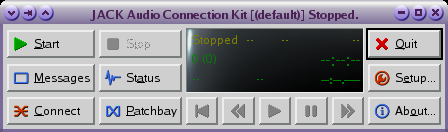
\includegraphics[scale=0.5]{images/qjack-stopped.png}}
\htmlonly{\image{0cm;0cm}{images/qjack-stopped.png}}
\caption{Main Control GUI of QJACKCTL}
\end{figure}


Next thing to do, is to click on the 'Start' button to launch the
(background) JACK sound server, and after a moment or two the QJACKCTL
control panel GUI should look like this ;


\begin{figure}
\latexonly{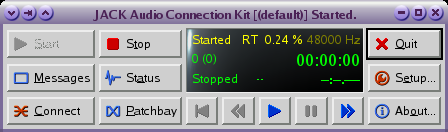
\includegraphics[scale=0.5]{images/qjack-running.png}}
\htmlonly{\image{0cm;0cm}{images/qjack-running.png}}
\caption{Main Control GUI of QJACKCTL}
\end{figure}


Now click on the 'Connect' button - this should open the connections
panel GUI. Click on the 'MIDI' connection tab - it should currently
look something like this ;

\begin{figure}
\latexonly{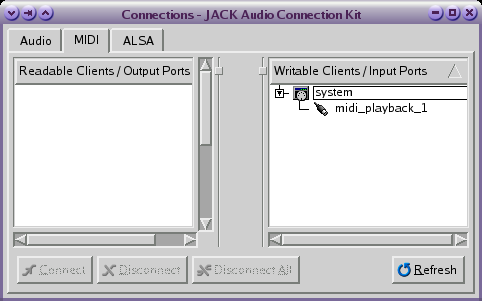
\includegraphics[scale=0.5]{images/qjack-connect-win-0.png}}
\htmlonly{\image{0cm;0cm}{images/qjack-connect-win-0.png}}
\caption{Connection  GUI of QJACKCTL}
\end{figure}


This all should have completed sucessfully and without generating any
errors or warnings. If this is the case, move onto the next step.


If however you have encountered errors or problems here, you will have to
fix them first before continuing -- JACK is an essential part of the
entire setup, and must be up and running properly before anything else
will work here. Look in the FAQ area of the manual Appendix for help with
common JACK/QJACKCTL errors and warnings. Once you get it all fixed, come
back and continue on here.


Step 4. The next step, is to start the actual synthesizer part itself.
In this example we are using the FLUIDSYNTH software synthesizer, which 
we control and configure using the QSYNTH frontend GUI you installed in
the beginning stages here. Look in your system's Multimedia or Sound menu
areas for the QSYNTH link and launch the program. If all has gone well this
far, QSYNTH will start and present you with it's main control GUI but the
actual softsynth itself will at this stage be unconfigured.


\begin{figure}
\latexonly{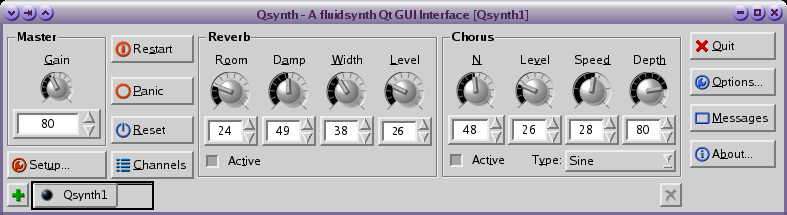
\includegraphics[scale=0.5]{images/qsynth-startup.png}}
\htmlonly{\image{0cm;0cm}{images/qsynth-startup.png}}
\caption{Main Control GUI of QSYNTH}
\end{figure}


Next thing to do, is configure the softsynth itself. Click on the 'Setup'
button in the main QSYNTH control GUI -- this will display the QSYNTH
configuration GUI. The first tab is the 'MIDI' setup page ;


\begin{figure}
\latexonly{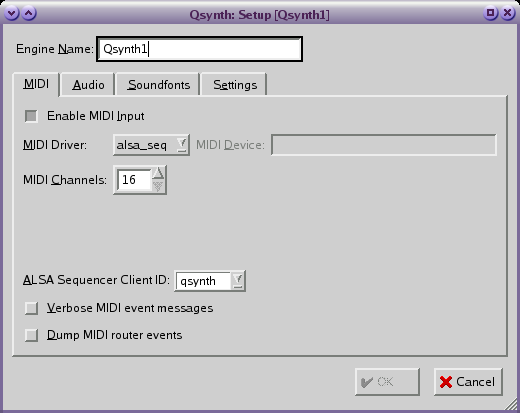
\includegraphics[scale=0.5]{images/qsynth-setup-0.png}}
\htmlonly{\image{0cm;0cm}{images/qsynth-setup-0.png}}
\caption{The MIDI Configuration GUI of QSYNTH}
\end{figure}



Your setup should look something closely akin to the above for using
a softsynth on Linux. Once you are happy with the settings, click on
the 'Audio' tab to display the Audio setup page ;



\begin{figure}
\latexonly{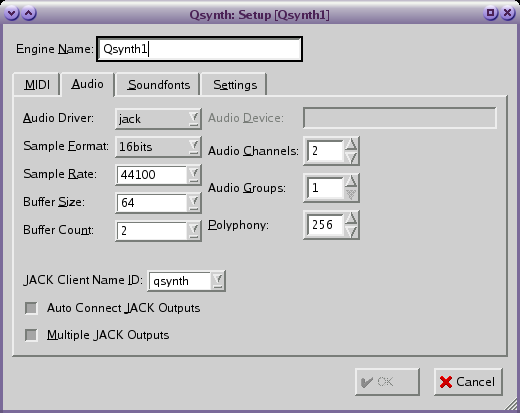
\includegraphics[scale=0.5]{images/qsynth-setup-1.png}}
\htmlonly{\image{0cm;0cm}{images/qsynth-setup-1.png}}
\caption{The Audio Configuration GUI of QSYNTH}
\end{figure}



Your setup should look something closely akin to the above for using
a softsynth on Linux using JACK as your audio output driver. This is
the most basic setup example - more complex environments are possible.
Once you are happy with the settings, click on the 'Soundfonts' tab to
display the Soundfont setup page - it should currently be empty ;


\begin{figure}
\latexonly{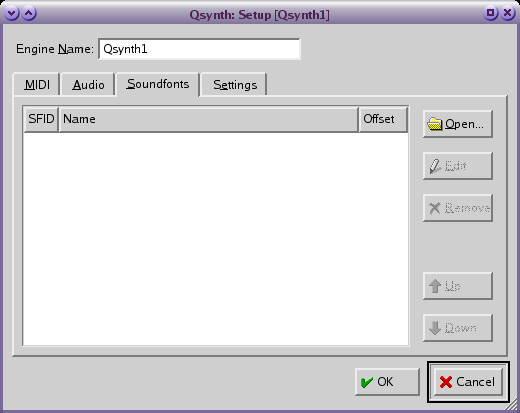
\includegraphics[scale=0.5]{images/qsynth-setup-2.png}}
\htmlonly{\image{0cm;0cm}{images/qsynth-setup-2.png}}
\caption{The Soundfont Configuration GUI of QSYNTH}
\end{figure}



This is a most important part of the softsynth setup - it is here you
define exactly what sounds (musical instruments, drum kits, sound FX,
synthesizer sound presets, etc, etc) your softsynth will be able to produce,
and how you do that is by loading (one or more) soundfont library files
into the softsynth itself, using this setup page. Click on the 'Open'
button, and a familiar looking 'open files' dialog window will appear ;



\begin{figure}
\latexonly{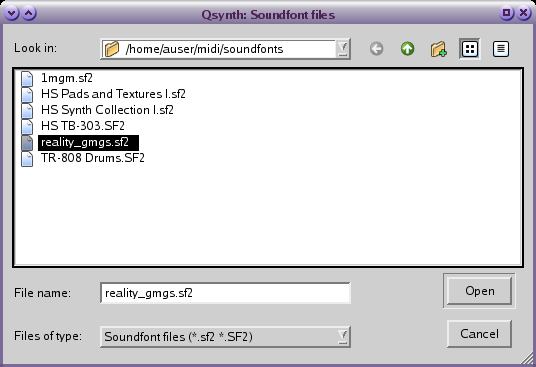
\includegraphics[scale=0.5]{images/qsynth-setup-3.png}}
\htmlonly{\image{0cm;0cm}{images/qsynth-setup-3.png}}
\caption{The Soundfont selection GUI of QSYNTH}
\end{figure}


Navigate to the location of the soundfont file you are going to use.
In the example you see above, the username 'auser' has created a
directory 'midi' in their HOME directory, and a 'soundfonts' directory
under that to keep their *.sf2 soundfont libraries in. Highlight the
soundfont file you wish to load, and then click on the 'open' button
This will load the selected soundfont library into the softsynth. Now
your Soundfont setup page should show that you've sucessfully loaded 
the soundfont library ;



\begin{figure}
\latexonly{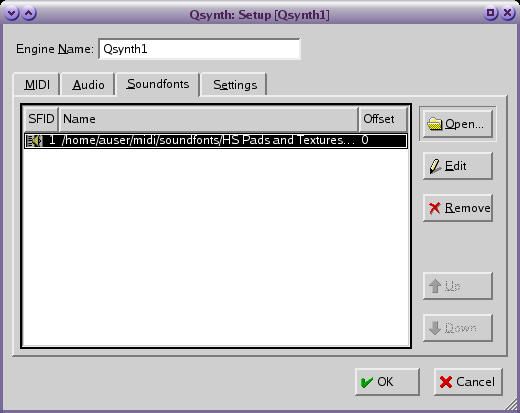
\includegraphics[scale=0.5]{images/qsynth-setup-4.png}}
\htmlonly{\image{0cm;0cm}{images/qsynth-setup-4.png}}
\caption{The Soundfont Configuration GUI of QSYNTH}
\end{figure}



If all has completed sucessfully so far, you're ready to move onto
the final step - starting Jazz++ itself. Before you do, you might
want to click on the 'Settings' tab, to get a quick reference of the
current synthesizer settings. Either way, once you are finished here,
click on the 'OK' button and continue onto the next step.



\begin{figure}
\latexonly{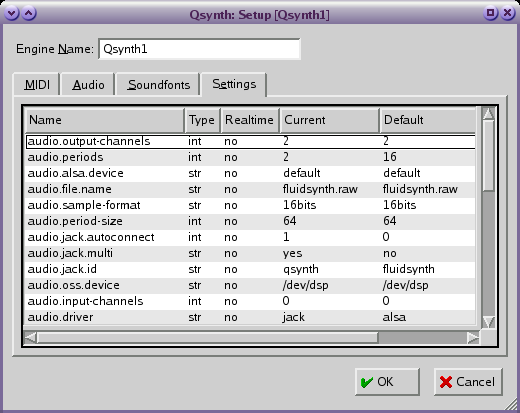
\includegraphics[scale=0.5]{images/qsynth-setup-5.png}}
\htmlonly{\image{0cm;0cm}{images/qsynth-setup-5.png}}
\caption{The Settings GUI of QSYNTH}
\end{figure}


Step 5. Now start Jazz++ itself (the jazz binary). If you have no 
currently configured MIDI input devices, Jazz++ will skip the MIDI 'input'
dialog window, and proceed directly to displaying  the MIDI 'output'
dialog window as exampled below ;



\begin{figure}
\latexonly{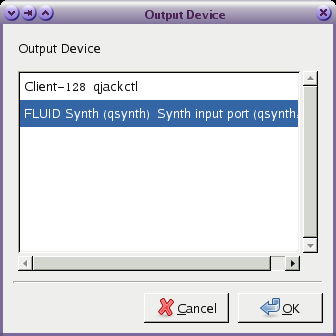
\includegraphics[scale=0.5]{images/jazz-output-sel-0.png}}
\htmlonly{\image{0cm;0cm}{images/jazz-output-sel-0.png}}
\caption{The Jazz++ MIDI Output Device selection GUI}
\end{figure}



Highlight the 'FLUID Synth (qsynth)' entry by clicking on it as in the
above example, then click on the 'OK' button. Jazz++ should now start
and present you with it's main track-window. Before you continue however,
you should check everything is 'connected' properly.

On the QJACKCTL control GUI, click on the 'Connect' button, and then
click on the 'Audio' tab. Expand the 'qsynth' and 'system' entries by
clicking on the little arrow to the left of their names. Your current
running configuration should appear like the example below ;



\begin{figure}
\latexonly{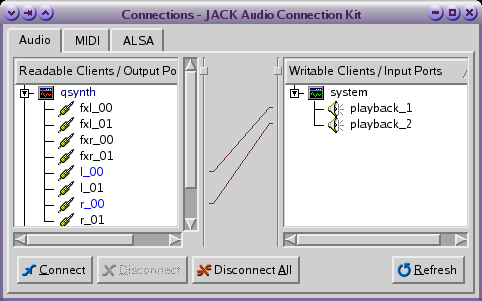
\includegraphics[scale=0.5]{images/qjack-connect-win-1.png}}
\htmlonly{\image{0cm;0cm}{images/qjack-connect-win-1.png}}
\caption{The Audio Connections GUI of QJACKCTL}
\end{figure}



Next, click on the MIDI tab in the same window, and ensure Jazz++ is
actually connected correctly as in the example below ;



\begin{figure}% 
\latexonly{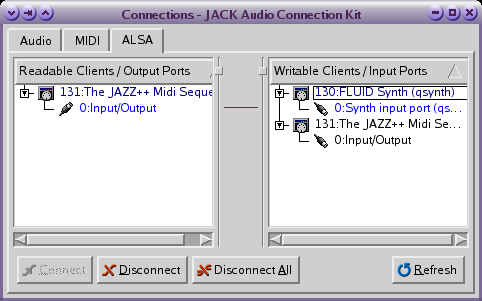
\includegraphics[scale=0.5]{images/qjack-connect-win-3.png}}% 
\htmlonly{\image{0cm;0cm}{images/qjack-connect-win-3.png}}
\caption{The MIDI Connections GUI of QJACKCTL}
\end{figure}



If all appears as exampled, you should be up and running. Load a song.mid
file into Jazz++ in the usual way, click on the play button and rejoice!



[ed: more to come here soon...my experience with the above instructions
-will- have things running, but whether the soundbank(s) get configured
correctly is another matter...still WIP here tho' ]


Still work in progress, come back soon!!



\section{Mac operating system}

[ed: help!!........]



\chapter{Overview of using Jazz++}\label{jazzwin}

[ed: fill this in later - see opening]

\chapter{Track window}\label{trackwin}

The trackwindow shows bars and tracks of your song while the
\helpref{pianowin}{pianowin} shows single events of one track. Events are shown like
bar codes, i.e. every event is shown as a short vertical line.

\begin{figure}
\latexonly{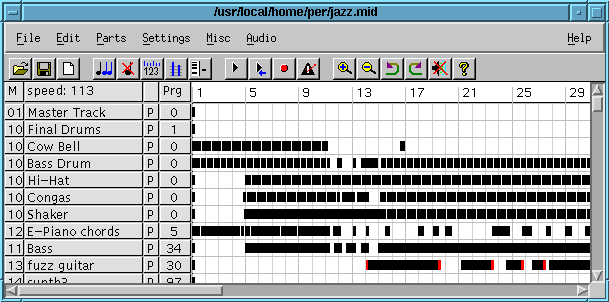
\includegraphics[scale=0.5]{trackwin.png}}
\htmlonly{\image{0cm;0cm}{trackwin.png}}
\caption{Track window}
\end{figure}


\section{Toolbar}\label{twtoolbar}

From left to right there are the following buttons:
\begin{enumerate}
\item \helpref{Open a file}{file}
\item \helpref{Save actual song to file}{file}
\item Clear song (start a new one)
\item \helpref{Replicate}{replicate}
\item \helpref{Delete}{delete}
\item \helpref{Quantize}{quantize}
\item \helpref{Mixer}{mixer}
\item \helpref{Piano Window}{pianowin}
\item \helpref{Play}{recplay}
\item \helpref{Loop play}{recplay}
\item \helpref{Record}{recplay}
\item \helpref{Metronome}{metro}
\item Zoom in
\item Zoom out
\item \helpref{Undo}{undo}
\item \helpref{Redo}{undo}
\item \helpref{Panic (MIDI reset)}{panic}
\item \helpref{Help}{twhelp}
\end{enumerate}

\begin{figure}
\latexonly{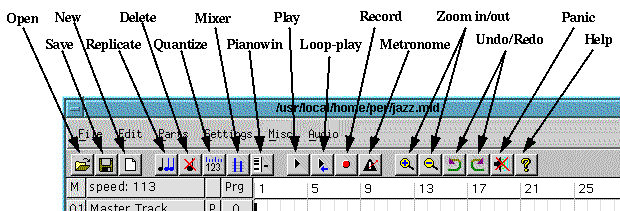
\includegraphics[scale=0.5]{twtoolb.png}}
\htmlonly{\image{0cm;0cm}{twtoolb.png}}
\caption{Track Window Toolbar}
\end{figure}

\section{Selecting events}\label{select}

Many functions (e.g 'Delete' from the edit menu) require that you have
selected some range of bars and tracks that will be affected by the
selected operation. You can drag a rectangle to select a range. Holding
the shift-key down while pressing the left mouse button will continue a
selection. This way, you can select a range bigger than the window by
continuing a selection after scrolling. Alternatively, you can click
into the leftmost column to select a whole track.

The selection indicates a range of tracks (y-axis) and a range of bars (x-axis).
These values are copied to the Event filter from Settings-Menu. In the event filter
you can specify more precise, which events shall be worked with.

Example: To delete all events but program changes from bar 5 to 15 on track 1 to 3,
mark bars and tracks by dragging a rectangle. Then select the event filter and
disable program-changes (patch). Finally select Delete from Edit-Menu.

\begin{figure}
\latexonly{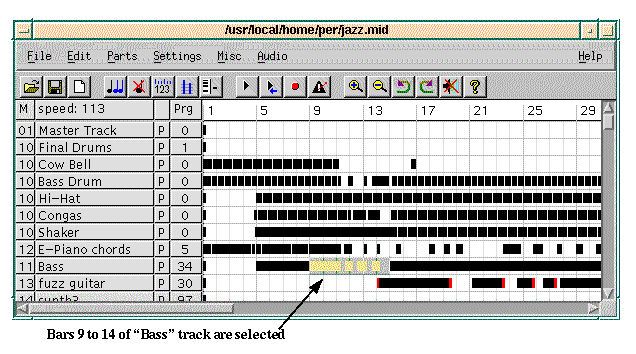
\includegraphics[scale=0.5]{twselect.png}}
\htmlonly{\image{0cm;0cm}{twselect.png}}
\caption{Selecting events}
\end{figure}

\section{Record and play}\label{recplay}

\begin{figure}
\latexonly{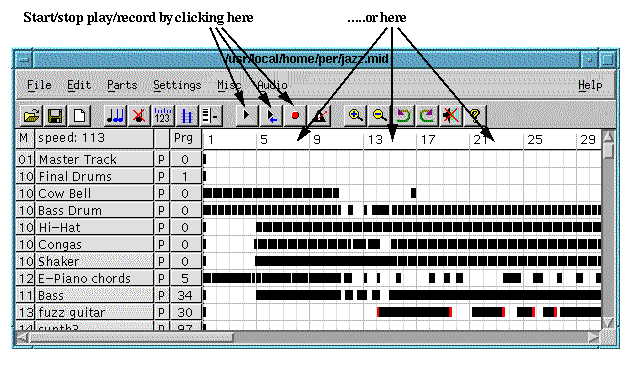
\includegraphics[scale=0.5]{recplay.png}}
\htmlonly{\image{0cm;0cm}{recplay.png}}
\caption{Record and play}
\end{figure}

There are 2 play modes
\begin{itemize}
\item {\em play} - normal linear play
\item {\em loop play} - requires that a loop-play range is selected (some bars in a track)
\end{itemize}

Each of the play modes has its own toolbar button. The buttons act both
as start-play and stop-play. After using JAZZ++ for a while you will
probably find it more convenient to start/stop play by clicking in the
top line of the Trackwindow. Play will then start at the bar where you click.
Loop play can also be done from the top-line by pressing shift-click.

Recording is done by pressing the record button after selecting
some bars in a track. The recorded events will be merged into the selection.
You can also start recording by clicking in the top-line of the Trackwindow
(some bars must be selected). If you start record with the right mouse button,
the track will be muted before play starts and existing events in the
selection will be replaced by the recorded events.

For a step-by-step tutorial on how to make a midi song from scratch, look at
\helpref{How to build a new midi song}{exmidisong}.

\section{Metronome}\label{metro}

The metronome button can be toggled on and off.
See also \helpref{Metronome settings}{metroset}.

\section{Speed adjustment}\label{speed}

A single click with left/right mouse button into the speed field will
increase / decrease the speed by one beat / minute. Keep the mouse button
down to make bigger changes. Hold down the shift key to change
values in steps of 10 bpm.

\begin{figure}
\latexonly{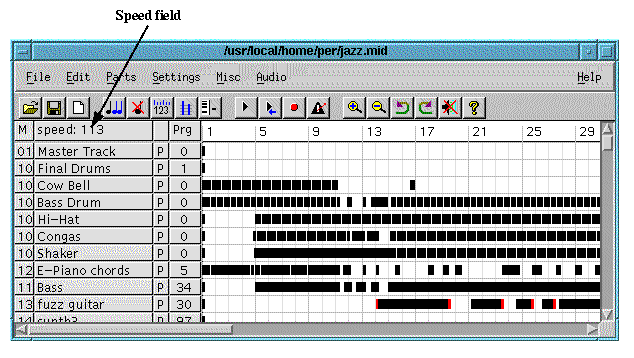
\includegraphics[scale=0.5]{speed.png}}
\htmlonly{\image{0cm;0cm}{speed.png}}
\caption{Speed adjustment}
\end{figure}


\section{Track Defaults (program, volume etc)}\label{trackdefs}

Clicking at the top of the column named Prg cycles through the available
defaults (Prg = program change, Bnk = program bank (used in combination
with Prg for GS and XG sounds), Vol = volume, Pan = pan, Rev = reverb,
Cho = chorus). These events are sent before play starts. To adjust a
value, click left or right mouse button to increase or decrease the
value (use the shift key for quick increase or decrease). A value of 0
means there is no event to be sent. Please note that the defaults can also be
edited (graphically) in the \helpref{Mixer dialog}{mixer} selected from the
\helpref{mixer toolbar button}{twtoolbar} or the {\em Parts} menu.

Clicking the unnamed column containing P's toggles the Trackstatus:
P=play, S=solo, M=mute.

Clicking into the top of the leftmost column (labeled 'M') toggles
display of midi channel and track number.

\begin{figure}
\latexonly{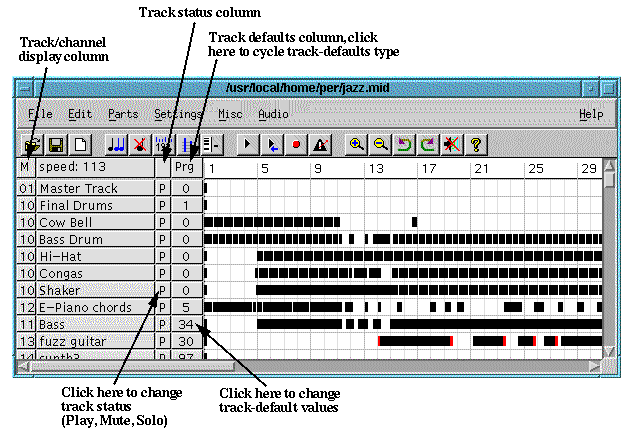
\includegraphics[scale=0.5]{trackdef.png}}
\htmlonly{\image{0cm;0cm}{trackdef.png}}
\caption{Track defaults}
\end{figure}

\section{Trackname, midi channel etc}\label{trackdlg}

Click on the name-field will open a Dialog. You can enter a new name for
the track, select the instrument to be played and define default midi channel.
If 'force all events to midi channel' is selected, all existing events on
the track will be set to the default midi channel when pressing 'Ok'.
Otherwise the midi channel will not affect events
already on the track.

\begin{figure}
\latexonly{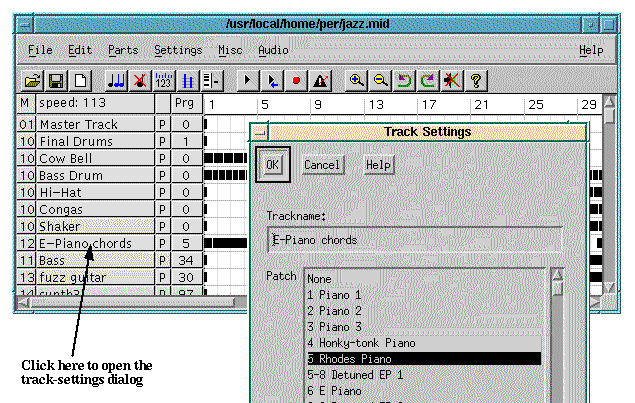
\includegraphics[scale=0.5]{tracknam.png}}
\htmlonly{\image{0cm;0cm}{tracknam.png}}
\caption{Track name, midi channel etc.}
\end{figure}


\section{Moving a whole track}

A whole track can be moved by clicking the right mouse button into the
track-name field, drag down/up to the destination and then release the
mouse button (drag and drop).


\section{File menu}\label{file}

\begin{itemize}
\item {\em Load, Save, Save As} - Load/Save MIDI-Standard files.
JAZZ++ will load both Format 0 and Format 1 midi files. Jazz always
saves Format 1 files.

\item {\em New} - Start editing a new song (clears the presently loaded
song). You will be asked for a file name when saving the new song.

\item {\em Load Template} is like normal load except that JAZZ++ will
treat the song as if it was a new song (you will be asked for a file
name when saved).

\item {\em Load Pattern} merges a midi standard file into the song. After
selecting the file, click with the left button to the destination position.
To abort loading after selecting the file click with the right mouse button
somewhere.

\item {\em Save Pattern} saves the selected events into a midi standard
file (Format 1).

\item {\em Quit} - exit JAZZ++.

\end{itemize}


\section{Edit menu}\label{twedit}


\subsection{Cut, Copy and Paste}\label{twclip}

This enables you to cut or copy some part of a song into an internal buffer
and paste it to another position of the song again. This can be used to
copy events from one song to another.

Do do this, \helpref{select}{select} some events and then select Cut or
Copy from the edit menu. To paste the events select paste from the edit menu
and click to the destination track/bar. To abort a paste operation click with
the right mouse button somewhere. Pasted events are merged with existing
events, so you may want to erase the destination tracks before pasting.



\subsection{Replicate}\label{replicate}

\begin{figure}
\latexonly{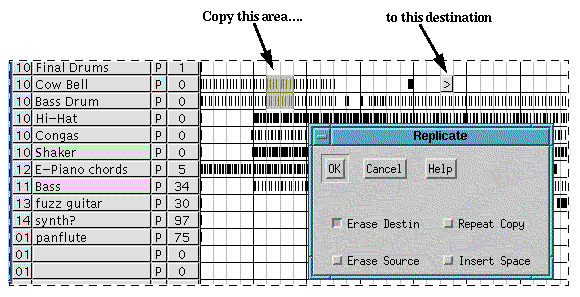
\includegraphics[scale=0.5]{replic.png}}
\htmlonly{\image{0cm;0cm}{replic.png}}
\caption{Replicate dialog}
\end{figure}

To replicate (copy) some events, you must first \helpref{select}{select}
an area. Then, after you have invoked {\em Edit$->$Replicate} (or
pressed the \helpref{replicate button}{twtoolbar}), your cursor will change to
a '$=>$', meaning that you should mark a
destination for the selected area (clicking with the right mouse button will
abort replication). After clicking destination position, you get a dialog
box. The meanings of the different check boxes are:

\begin{itemize}
\item {\em Erase Destin}

\begin{itemize}
\item {\em Checked} - destination will be replaced by source
\item {\em Unchecked} - events will be merged
\end{itemize}

\item {\em Erase Source}. Source will be moved to destination

\item {\em Repeat Copy}. After clicking Ok, you can click at the end of the
destination range. Repeated copies of source will fill the destination range.

\item {\em Insert Space}. All Events right from the destination point will
be moved to the right to make room for the copied events.

\end{itemize}

Source and Destin may overlap.



\subsection{Delete}\label{delete}

\begin{figure}
\latexonly{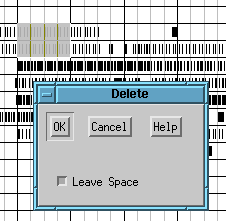
\includegraphics[scale=0.5]{delete.png}}
\htmlonly{\image{0cm;0cm}{delete.png}}
\caption{Delete dialog}
\end{figure}

To delete some events, you must first \helpref{select}{select} an area.
Then, after you have invoked {\em Edit$->Delete$} (or pressed the
\helpref{delete button}{twtoolbar}), you get a
dialog box. The check box 'Leave space' has the following meaning:

\begin{itemize}
\item {\em checked} - the deleted events leave a hole
\item {\em unchecked} - the events from right are moved to the left to
fill up the hole
\end{itemize}


\subsection{Quantize}\label{quantize}

Quantize will put Note-On events in the selected area 'in time' (moved to the
nearest step-timing value). Only Note-On events are changed.

\begin{figure}
\latexonly{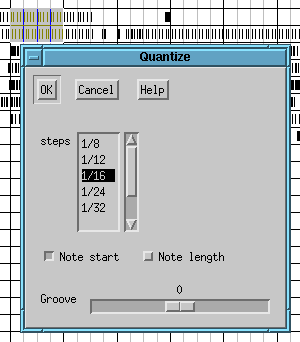
\includegraphics[scale=0.5]{quantize.png}}
\htmlonly{\image{0cm;0cm}{quantize.png}}
\caption{Quantize dialog}
\end{figure}

To quantize some events, you must first \helpref{select}{select} an area.
Then, after you have invoked {\em Edit$->$Quantize} (or pressed the
\helpref{Quantize button}{twtoolbar}), you get a
dialog box. The 'steps' listbox represent the 'granularity' of the
quantization, and should normally correspond to the smallest note-timing
value of the music to be quantized. The checkboxes control whether the
start of the note or the end of the note (or both) should be quantized.

There is also a slider named 'Groove' that can be used for quantizing notes
'off beat'. A value of e.g. +20 means that the notes are moved to the nearest
step-timing plus 20 percent of a step-value (notes will sound a bit 'late'). A
negative value will make notes sound a bit 'early'. For normal quantization
the value should be 0.


\subsection{Set MIDI Channel}\label{setchan}

The selected events will be set to the selected MIDI Channel.

\begin{figure}
\latexonly{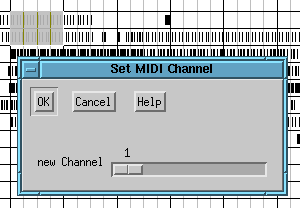
\includegraphics[scale=0.5]{setchan.png}}
\htmlonly{\image{0cm;0cm}{setchan.png}}
\caption{Set MIDI channel dialog}
\end{figure}


\subsection{Transpose}\label{transpose}

\begin{figure}
\latexonly{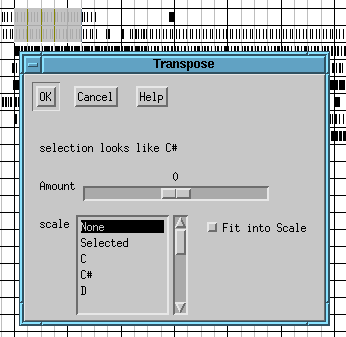
\includegraphics[scale=0.5]{transpos.png}}
\htmlonly{\image{0cm;0cm}{transpos.png}}
\caption{Transpose dialog}
\end{figure}

If no scale is selected, Amount is the number of semitones to transpose, e.g. an
Amount of 1 will change C to C\#, C\# to D etc. If the scale C is selected, C
will become D, D will become E, E will become F etc. JAZZ++ tries to analyze
the key of the selection and displays it in the dialog.

The scale 'selected' is the set of notes in the selection. If eg the selection
contains the notes C, D, E an amount of 1 will change C's to D's, D's to E's and
E's to C's. Its useful in the piano window create inversions of chords.

Fit into scale with an amount of 0 will change all notes to the nearest one
contained in the selected scale. If eg the selection contains some C\# and you
select C scale, all C\#'s will become C's (D would be possible too, but transpose
down is preferred in this case). If amount is not 0, the selection is transposed
in semitones first and 'Fit into scale' afterwards.

Only Note-On events are changed.


\subsection{Velocity}\label{veloc}

\begin{figure}
\latexonly{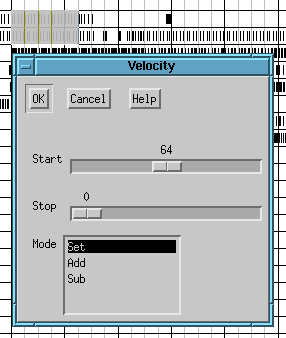
\includegraphics[scale=0.5]{veloc.png}}
\htmlonly{\image{0cm;0cm}{veloc.png}}
\caption{Set velocity dialog}
\end{figure}

Changes the velocity of Note-On events. If Stop is 0, all Note-On events will get
the Start velocity. If Stop is greater 0, events at the beginning of the selection
will get the Start velocity, those at the end will get the Stop velocity
(e.g. crescendo). The choice Add/Sub/Set determines, how the value is applied.


\subsection{Length}\label{length}

Adjust length of Note-On events. see \helpref{Velocity}{veloc}.


\subsection{Shift}\label{shift}

\begin{figure}
\latexonly{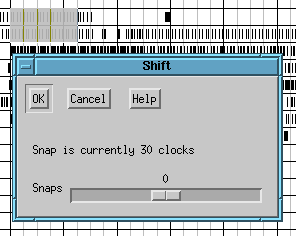
\includegraphics[scale=0.5]{shift.png}}
\htmlonly{\image{0cm;0cm}{shift.png}}
\caption{Shift dialog}
\end{figure}

Moves events left or right in amounts smaller than a bar. The snap value is
adjusted in the pianowin.

\subsection{Cleanup}\label{cleanup}

\begin{figure}
\latexonly{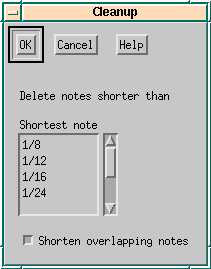
\includegraphics[scale=0.5]{cleanup.png}}
\htmlonly{\image{0cm;0cm}{cleanup.png}}
\caption{Cleanup dialog}
\end{figure}

Deletes note-on events that are shorter than a selected length. Optionally
shorten notes to insure that notes of the same pitch does not overlap.

Accidental keyboard hits often leave very short notes on the track that
distorts the music. Another problem is that two overlapping notes of the
same pitch causes the second note to stop sounding (because of the note-off
event from the first note). This cleanup function effectively solve such
problems.

\subsection{Search Replace}\label{search}

\begin{figure}
\latexonly{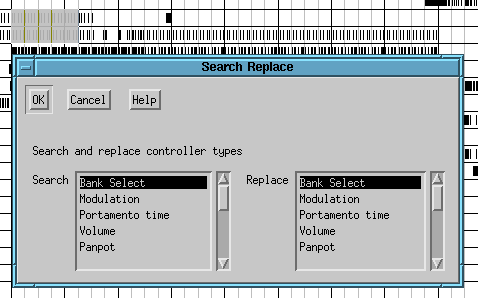
\includegraphics[scale=0.5]{search.png}}
\htmlonly{\image{0cm;0cm}{search.png}}
\caption{Search Replace dialog}
\end{figure}

Searches for controller events and changes the controller number, eg
transforms modulation wheel to volume.




%%%%%%%%%%%%%%%%%%%%%%%%%%%%%%%%%%%%%%%%%%%%%%%%%%%%%%%%%%%%%%%%%%%%%%%%%

\section{Parts menu}\label{partsmenu}

This menu deals with all kinds of instrument settings, or {\em parts} settings.
Some of the parameters will work with
almost any General Midi (GM) equipment (like Volume settings) while
others only work with GS- or XG-compatible synthesizers. The number of
selectable menu entries will vary depending on the
\helpref{synthesizer type}{synthtype} settings.

Please note that some
menu entries may have no effect on your equipment even if selectable. In some
cases special {\em system exclusive} message needs to be sent
first in order to enable the specific feature
(see \helpref{Edit/create single events}{pweventedit} on how to create a
system exclusive event).
In other cases the equipment just doesn't support the feature.
Please consult the owner's manual of your sound generator for more info.

All parameters are operated with sliders per track (part). Note that for some
platforms the number of adjustable parameters are restricted because of
the size of the dialogs.

Please note that only one {\em parts} dialog can be opened at a time.

\subsection{Mixer and Master}\label{mixer}

Setting of default {\em Volume}, {\em Pan}, {\em Reverb} and {\em Chorus}.

\begin{figure}
\latexonly{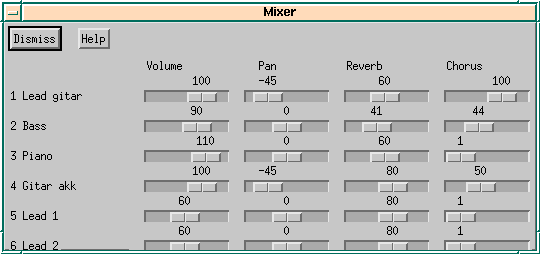
\includegraphics[scale=0.5]{mixer.png}}
\htmlonly{\image{0cm;0cm}{mixer.png}}
\caption{Mixer window}
\end{figure}

\subsection{Sound, Vibrato and Envelope}

Sound dialog - change sound color:

\begin{itemize}
\item {\em Cutoff frequency} - filter high frequencies
\item {\em Resonance} - make the sound more 'synthetic' (wha-wha sound)
\end{itemize}

Vibrato dialog - change the way the tone's vibrato develops in time:

\begin{itemize}
\item {\em Vibrato Rate} - controls how fast the vibrato will be
\item {\em Vibrato Depth} - controls how much vibrato you get
\item {\em Vibrato Delay} - controls at what time after note start the
vibrato begins
\end{itemize}

Envelope dialog - change the way the tone envelope (amplitude) develops in
time:

\begin{itemize}
\item {\em Envelope Attack} - controls how fast the tone increases in volume
when it starts
\item {\em Envelope Decay} - controls how fast the tone will
decrease in volume after it has started (also called {\em sustain})
\item {\em Envelope Release} - controls how fast the tone decreases in volume
after it is has ended (how fast the tone stops)
\end{itemize}

\subsection{Controller dialogs}
These dialogs change the way the different controllers affect the sound.

Controllers are:

\begin{itemize}
\item {\em Pitch Bender} - used to control continuous tone-pitch in real time
\item {\em Modulation Wheel} - used to control 'tone expression'
(e.g. vibrato) in real time
\item {\em Channel Aftertouch (CAf)} - some keyboards senses how hard you
press down the key after the attack, used for 'tone expression' in real
time. Affects all tones of the part (midi channel).
\item {\em Polyphonic Aftertouch (PAf)} - same as above, but only affects
one key pitch of a part (channel).
\item {\em Continuous Controller 1 (CC1)} - used for misc. 'tone expression'
\item {\em Continuous Controller 2 (CC1)} - used for misc. 'tone expression'
\end{itemize}

All the controllers have three associated types dialogs with sliders;
{\em Basic}, {\em LFO1} and {\em LFO2}.
The settings tell how much the controller will trigger the
sound-change described by each parameter. Parameters are:

\begin{itemize}
\item {\em Pitch Control / Sense} - pitch in half-tone steps
\item {\em TVF Cutoff} - controls high frequency cutoff (TVF =
Time Variant Filter)
\item {\em Amplitude} - controls amplitude (dynamic volume)
\item {\em LFO1 Rate, Pitch, TVF and TVA} - controls the rate of the Low
Frequency Oscillator 1 (LFO1) and how it affects pitch, TVF and TVA (TVA =
Time Variant Amplitude)
\item {\em LFO2 Rate, Pitch, TVF and TVA} - controls the rate of the Low
Frequency Oscillator 2 (LFO2) and how it affects pitch, TVF and TVA (TVA =
Time Variant Amplitude)
\end{itemize}

The {\em Basic} dialogs of the {\em Continuous Controller} entries also has
a {\em Controller Nr} dialog to set what continuous controller the part
will respond to.


\subsection{Drum Instrument Parameters}

This is a dialog for controlling different parameters of the individual drum
instruments of the primary drum part. The track selected is the first track
with channel equal to the {\em .drumchannel} setting (in the configuration
file ). Note that the name of the track also has to be set.

Drum instruments are listed in a list box. The sliders are valid for the
instrument currently selected from the list. Listed instruments to be
controlled are added/deleted by using the {\em Add} and {\em Del} buttons.

The controllable parameters are:

\begin{itemize}
\item Drum instrument {\em pitch coarse}
\item Drum instrument {\em TVA} (volume)
\item Drum instrument {\em panpot} (checkbox gives random pan)
\item Drum instrument {\em reverb send}
\item Drum instrument {\em chorus send}
\end{itemize}


\subsection{Partial Reserve}

Sound generators have a limited amount of tones that can be played
simultaneously. This is sometimes referred to as 'maximum polyphony'.
When the maximum polyphony is exceeded the synthesizer will start
cutting tones, which can cause audible 'distortion' to the music.

In some GS equipment you can assign the number of tones (oscillators)
that is assigned to each part (channel) and thereby control which instruments
are 'more important'. This is what this dialog is for.

\subsection{Part Mode}

Here you can set two things:

\begin{itemize}
\item {\em Rx Channel} - the channel to be received by the part
\item {\em Use for rhythm} - sets the part to normal mode (value 0)
or drum modes (value > 1). Part 10 (channel 10) has default value 1,
all others have default value 0. On GS and XG synths you can get another drum
part by setting that part to value > 1.
\end{itemize}

%%%%%%%%%%%%%%%%%%%%%%%%%%%%%%%%%%%%%%%%%%%%%%%%%%%%%%%%%%%%%%%%%%%%%%%%%
\section{Settings menu}\label{twsettings}

\subsection{Filter}\label{midifilter}

Using the 'event filter dialog', you can specify what types and ranges of
events that will be affected by \helpref{selection}{select} operations like
e.g. 'Delete' and 'Replicate'.

\begin{figure}
\latexonly{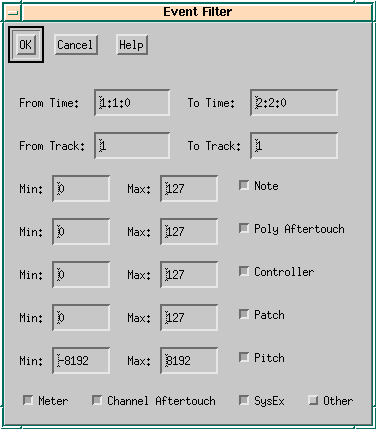
\includegraphics[scale=0.5]{filter.png}}
\htmlonly{\image{0cm;0cm}{filter.png}}
\caption{Event filter dialog}
\end{figure}

The entries {\em From Time}, {\em To Time}, {\em From Track} and
{\em To Track} are automatically set by selecting a range with the mouse.

The checkboxes {\em Note}, {\em Controller}, {\em Patch} (Program Change),
{\em Pitch}, {\em Meter} and {\em Other} decide whether these event types
should be included in the selection. For the first four event types you can
also specify more closely which values will be included.

By default, all 'boxes' except {\em Other} are checked, leaving e.g.
{\em Tempo} events unchanged by selection operations.

\subsection{Window}
adjust size of fonts (y-axis) and events (x-axis).



\subsection{Song}\label{songset}

\begin{figure}
\latexonly{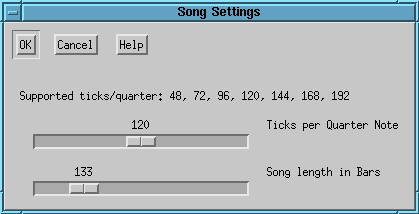
\includegraphics[scale=0.5]{songset.png}}
\htmlonly{\image{0cm;0cm}{songset.png}}
\caption{Song settings dialog}
\end{figure}

Here you can adjust the overall resolution of the song in ticks per quarter.
The native JAZZ++ driver (MPU-401) supports distinct values only. With OSS
and on MS-Windows you can use any value here. If you change this value,
all event timings are recomputed.

A big value of 'ticks per quarter' means that the time resolution of the
notes in the song will be better, but the strain on the sequencer system
will also increase. Many people think it is important to have a big value here,
while others say you won't hear the difference. We recommend you to use
the default value (120 ticks per quarter) which gives sufficient resolution
for any 'normal' midi song.

In this dialog you may also set the maximum length of the song in bars.
This value is used to set the scrollbars in the track and piano windows.


\subsection{Metronome Settings}\label{metroset}

\begin{figure}
\latexonly{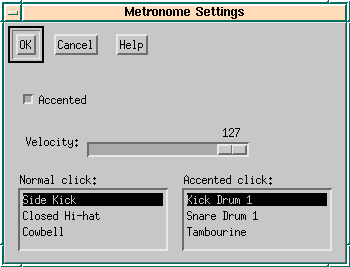
\includegraphics[scale=0.5]{metroset.png}}
\htmlonly{\image{0cm;0cm}{metroset.png}}
\caption{Metronome settings dialog}
\end{figure}

Adjust metronome instruments and velocity.

An ``accented'' metronome means that the first count of a bar sounds different
than the other counts.

\subsection{Effects}

Adjust GS or XG effect settings. In XG mode, also equalizer settings can be
chosen.

In GS mode, effects can be adjusted in two modes dependent on the settings
of the 'Use effect macro' and 'Use chorus macro' checkboxes:
\begin{itemize}
\item {\em macro mode} - the choices in the macro listboxes are valid
\item {\em individual parameter mode} - the values of the parameter
sliders are valid
\end{itemize}

Macro mode will be sufficient in most practical cases. Setting of individual
parameters is more difficult, but can give very good results when done right.

The mode settings (position of the checkboxes) can be saved with the
"Save settings" menu entry. The current values of the listboxes or parameter
sliders are stored in the midi file.

\subsection{Timing}

Controls clock source and real-time output.

The available choices of {\em clock source} will vary depending on system
platform:

\begin{itemize}

\item {\em Internal}. The sequencer is itself the source of the clock timing
(available on all system platforms).

\item {\em Song Pointer}. The sequencer clock locks to midi real-time messages
received from midi input. The source of these messages is typically a
tape-machine with an external sync-box or just another sequencer. Song
pointer sync is available on Unix with JAZZ++-native MPU-401 driver and on
MS-Windows.

\item {\em Midi Time Code}. The sequencer clock locks to Midi Time Code
(MTC) messages received from midi input. The source is typically a
tape-machine with an external sync-box doing SMPTE-to-MTC conversion or
a MTC-capable recording machine. MTC sync is available on MS-Windows platform.

\item {\em FSK}. The sequencer clock locks to FSK information received from
tape. This is available on Unix with an MPU-401 card supporting FSK
sync.

\end{itemize}

How to sync?

\begin{itemize}

\item {\em Internal}.
Just play; JAZZ++ is the master and decides all timing
using internal clocks in the computer.

\item {\em Song Pointer}.
Make sure the device (here called "tape") you are syncing
to sends midi real-time messages (songpointer, midi clock etc.) This could
involve recording a "songpointer stripe" to a tape track by means of
a sync box. To do this you must play the song with the sequencer in
"Internal" sync mode and with "Realtime to MIDI Out" enabled. (For more info
refer to the instructions of the sync box.)

To play, enable "Song pointer" sync mode in sequencer (JAZZ++), start play on
sequencer
first, then start tape at any point in the song. The sequencer is now locked
to the movements of the tape. (Note that some sync boxes don't send
song-pointer at beginning of the song. In this situation you must manually
start sequencer at song-start before running tape.)

\item {\em Midi Time Code}.
Make sure the device (tape) you are syncing to sends
MTC messages (could involve recording an SMPTE stripe). Set the MTC offset
and the MTC type either manually or by recording it while listening to the
tape. (The MTC offset is the point in time when the sequencer is supposed
to start playing the song.) When recording MTC offset the sequencer will
automatically be set into MTC sync mode.

To play, set sequencer to MTC sync mode, start play on sequencer, then start
tape at any point in the song. The sequencer is now locked to the movements
of the external device.

\item {\em FSK}.
An "FSK stripe" must first be recorded to a tape track. To do
this you must play the song with the sequencer in "Internal" sync mode. Be
sure to start FSK stripe recording some time before sequencer is started
(must record the pilot tone).

To play, set sequencer to FSK sync mode, start tape in the pilot-tone area,
then start sequencer before pilot tone ends. (Note that with FSK play must
always start at beginning of the song.)

\end{itemize}

The "Realtime to Midi Out" choice is useful for syncing another sequencer
to this one or to record a "songpointer stripe" to tape via a sync box.
Note that "Realtime to Midi Out" will only work properly for a
ticks-per-quarter resolution dividable by 24
(see \helpref{Song settings}{songset}).


\subsection{Midi Thru}
Enable/disable midi thru. Should normally be enabled.

When enabled, the sequencer will send all notes received on
the MIDI IN port to the MIDI OUT port. This basically means that you will hear
what you play on the keyboard.

\subsection{Synthesizer Type Settings}\label{synthtype}

\begin{figure}
\latexonly{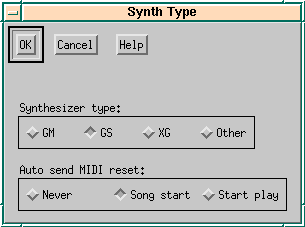
\includegraphics[scale=0.5]{syntype.png}}
\htmlonly{\image{0cm;0cm}{syntype.png}}
\caption{Setting of synthesizer type}
\end{figure}

Many MIDI sound generators (a synthesizer, soundmodule or soundcard) offer
possibilities to choose an extended number of instruments (more than
the 128 General MIDI instruments), or to control things like sound colour,
reverb/chorus settings or time-variant filters. This is done by sending
specific MIDI commands from the sequencer
(bank-, NRPN- and SYSEX-events). However, the parameters of
these commands are different depending on which standard your sound
generator supports.

To allow JAZZ++ to get the most out of your MIDI sound generator, you should
choose the synthesizer type option that corresponds most closely to your
equipment.

Options are:

\begin{itemize}

\item{\em GM}
- Choose this if your sound generator is a standard General MIDI device.
This option is safe and will work for almost any sound generator.

\item{\em GS}
- GS is an extension to the GM specification that allows for 317 different
instruments, effect type control and a lot more. Look for the GS logo on
your equipment. GS was originally defined by Roland (R).

\item{\em XG}
- XG is another extension to GM. A lot of extra instruments
are defined as well as a number of extended control possibilities. Look
for the XG logo on your equipment. XG was originally defined by
Yamaha (R).

\item{\em Other}
- This option is for sound generators that do not follow any of the standards
mentioned above. JAZZ++ allows user customization of parameters like
instrument lists (patches), controllers and drum instrument names. Look
into the JAZZ++ \helpref{configuration files}{installation} for more info.

\end{itemize}

The 'Auto send MIDI reset' options control the conditions for when JAZZ++
should send a MIDI reset command (corresponding to the synthesizer type) to the
synthesizer device.

\begin{itemize}
\item {\em Never} - MIDI reset is never automatically sent to the device
(only when you press the \helpref{panic putton}{twtoolbar})
\item {\em Song start} - MIDI reset is sent whenever play starts from the
beginning of the song (default)
\item {\em Start play} - MIDI reset is always sent when play starts
\end{itemize}

Files saved from JAZZ++ will always contain a MIDI reset near the beginning
of track 0.

\subsection{Midi Device}

You may select the input and output devices from the list of installed
drivers.

\subsection{Save Settings}
Save settings to config file.
Affected settings: midi thru, clock source, realtime out, effect macro modes,
display welcome message and window geometry.


\section{Misc menu}

\subsection{Undo and redo}\label{undo}

Undo or redo the last operation. The last 20 operations can be undone/redone.


\subsection{Merge / Split Tracks}

{\em Split tracks} places all events from track 0 to track 1..16 depending on
the midi channel (useful for 'decoding' a format 0 midi file).

{\em Merge tracks} moves all events to track 0 (not so useful as JAZZ++ only
saves file format 1).

\subsection{Meterchange}\label{meterchange}

\begin{figure}
\latexonly{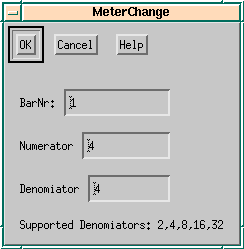
\includegraphics[scale=0.5]{meter.png}}
\htmlonly{\image{0cm;0cm}{meter.png}}
\caption{Meter change dialog}
\end{figure}

Changes the meter (counts per bar and note-value of each count) starting
from specified bar to the end of song or to the
next meterchange. {\em Numinator} is the 'counts per bar', while
{\em Denominator} is the 'note-value of a count'.

Meterchange events are placed on track 0 always.

\subsection{Midi reset}\label{panic}

Sends an initialize message (either 'GM ON', 'GS ON' or 'XG ON') to the midi
port. If \helpref{synthesizer type}{synthtype} is correctly set, most sound
generators will initialize to default values when such a message is
sent.

\subsection{Harmony browser}\label{hbrowser}

\begin{figure}
\latexonly{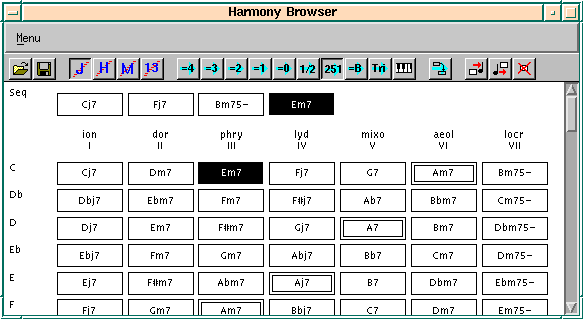
\includegraphics[scale=0.5]{hb.png}}
\htmlonly{\image{0cm;0cm}{hb.png}}
\caption{Harmony browser}
\end{figure}

\begin{figure}
\latexonly{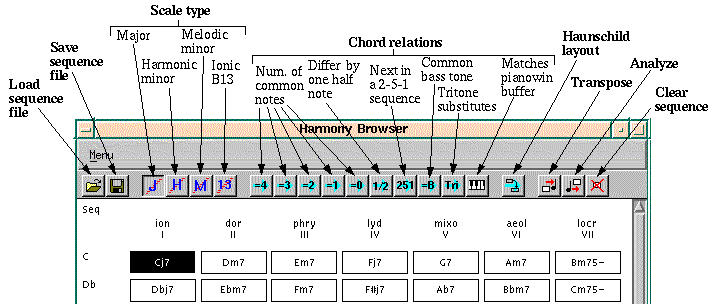
\includegraphics[scale=0.5]{hbtoolb.png}}
\htmlonly{\image{0cm;0cm}{hbtoolb.png}}
\caption{Harmony browser toolbar}
\end{figure}

The harmony browser shows the 4-tuned JAZZ++ harmonies of the four scales
types major, harmonic minor, melodic minor and harmonic major.

The first thing you can do is to click on chords and listen how they sound (eg
examples from a song book or a book about harmony theory). The selected
chord is placed into the pianowin copy buffer and can be pasted into
your song (see \helpref{mouse actions}{mouseact}.

The harmony browser is also able to analyze a section of your song and
to transpose parts of your song into new scales and chords. Also you may generate
chords thru the random rhythm generator into your song.

What you can do with the mouse:
\begin{itemize}
\item {\em left click on a chord} selects the chord and marks related chords (see below).
\item {\em shift + left} click selects the chord and appends it to the chord sequence
you need to transpose parts of your song
\item {\em right click} just listen to the chord, don't select it
\item {\em right click on the last chord} of the chord sequence removes this
chord from the sequence.
\end{itemize}

There is a toolbar with the following icons (from left to right):

\begin{itemize}

\item {\em The left four buttons} switch the scale type for which the standard
chords are displayed: major, harmonic minor, melodic minor and harmonic
major which is also known as ionic b13.

\end{itemize}

The following five Icons (with the cyan right arrow and the piano)
specify what related chords are marked when you select a chord:

\begin{itemize}

\item {\em 4,3,2,1,0} marks all chords that have 4,3,2,1,0 common notes with the
actual chord

\item {\em 1/2} marks all chords, that differ from the selected chord by exactly
one half note

\item {\em 251} marks all chords, that would come next in the 2-5-1 move

\item {\em =B} marks all chords, that share the same bass note with the selected chord

\item {\em Tri} marks all chords, that could be tritone substitutes (their bass note
is at a tritone interval from the selected chord).

\item {\em (piano)} mark all chords, that contain all of the keys in the pianowin
copy buffer. So you could select a few notes (max 4) in the pianowin and select
copy from the edit menu. Now the harmony browser will mark all chords that contain
those notes.

If the piano button is not selected, the harmony browser works the other way round.
Whenever you select a chord, the chord is placed into the pianowin buffer so you
can paste it into your song. The parameters (midi channel, length etc) can be set
in the midi-entry of the harmony browser menu.

\end{itemize}

The last four buttons do different things:

{\bf Haunschild layout} shows harmonies and scales in an order proposed
in a book about harmony theory by the German author Haunschild. If selected,
chords are shown in a way that 'valid moves' are

\begin{itemize}
\item {\em from left to right}, e.g the 2-5-1 move is displayed as three neighbored
chords. In general, all horizontal moves are allowed.
\item {\em vertical moves} are allowed, they change one semitone of a chord (at most).
\item {\em diagonal} from top-left to bottom right. I don't know why, but it sounds
nice.
\end{itemize}

{\bf Transpose} lets you change parts of your song to the harmonies and chords
of the chord sequence. When you select some bars in the trackwin and
click on transpose, then the selection is mapped to the chord sequence.
The default is, that on chord lasts one bar, but you may change this in the
settings menu in the harmony browser. If the results are not satisfying, you
should try to transpose track by track, this often works better. All in all,
transposing works better, when the selected material is not too complicated.

I had nice results with the following procedure: I recorded (very slow, as I am
not a good piano player) cj7 chords on one track, some monphone bass line on the
second track and a solo on the third track. Everything was in c major (white keys
only). Then I selected some chords and transposed each track on its own.

{\bf Analyze} Tries to find the chords and scales from the selection in the
trackwin. Again, the default is one harmony per bar which can be changed in the
settings menu. The algorithm looks at the length of the notes and chooses the
longest notes to be the notes of the chord.

{\bf Clear chord sequence} removes all chords from the chord sequence.


{\bf Menu entries}

\begin{itemize}
\item {\em edit chord} - often you may want to have chords/scales that are not displayed
in the harmony browser. You can select a chord from the chord sequence and change
it in this dialog.

\item {\em settings} - adjust parameters for transpose and analyze as explained above.
A value of 0 quarters per chord when transposing will map the chords to the length
of the selection, e.g if you have selected 16 Bars and your sequence has 4 chords,
every chord will last 4 bars. If you had chosen 4 quarters instead, the chord
sequence would have been repeated 4 times to fill the 16 bars of the trackwin selection.

\item {\em midi} - these settings affect what you hear, when clicking on a chord and what
is put into the pianowin buffer.

\end{itemize}

{\bf Generating chords with the random rhythm generator}

After defining a chord sequence, you may open the random rhythm
generator. When adding an instrument, it will show (beside drums) the
instrument 'chords from harmony browser'. You select it and define a more or
less randomized rhythm and proceed as described \helpref{here}{randrhy}.

\subsubsection{Transpose Algorithm}

This one is somewhat difficult to explain, but its probably the most
interesting feature of the Harmony Browser.  Lets assume, you have a
sequence of 4 chords. Then you select 4 bars in the track window (all
tracks) and you press the transpose button.  Now, the Harmony Browser
tries to change the harmonies and scales from the trackwindow selection
into the selected chords.

The algorithm looks at the first bar from the trackwin selection and
sums up the length of all different notes. It assumes, that the 4 notes with the
largest sum of length are the chords present in the song and changes them
to the 4 notes from the first chord of your chord selection. Afterwards,
the remaining notes from the trackwin selection are mapped to the remaining
notes of the scale the chord was taken from.



\subsection{Random rhythm generator}\label{randrhy}

\begin{figure}
\latexonly{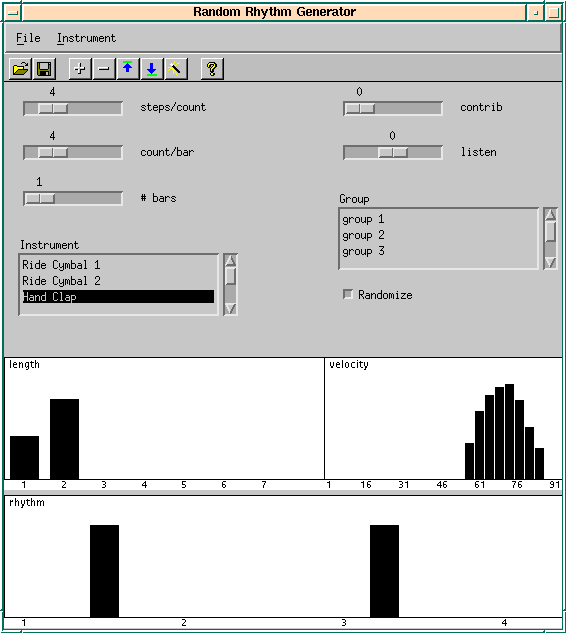
\includegraphics[scale=0.5]{rrg.png}}
\htmlonly{\image{0cm;0cm}{rrg.png}}
\caption{Random rhythm generator}
\end{figure}

\begin{figure}
\latexonly{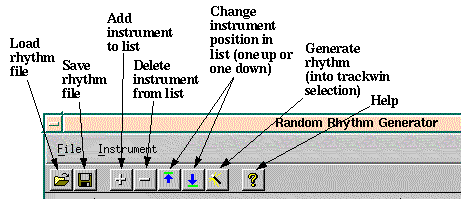
\includegraphics[scale=0.5]{rrgtoolb.png}}
\htmlonly{\image{0cm;0cm}{rrgtoolb.png}}
\caption{Random rhythm generator toolbar}
\end{figure}

This dialog generates rhythms from some kind of statistical specification.
You define probabilities for timing, velocity and note-length and from these
the rhythm is generated.

With the three sliders you specify the meter and (with \# Bars) how many
probabilities you want to define. Next, you can add or remove instruments
to the listbox. Then you specify the probabilities for rhythm, velocity
and length for each instrument.

Probabilities are set with the mouse where

\begin{itemize}
\item {\em left button} - draw some kind of curve
\item {\em right button} - clear values to zero
\item {\em + shift} - adjust all values simultaneously
\item {\em + ctrl} - adjust exactly one value
\end{itemize}

In the rhythm field you specify the probabilities for every time
position. A high value means a high probability that the instrument is
played definitely at that time. A low value means, that the instrument
{\em may} be played at that time. By adjusting high values only, you
can specify a definite rhythm without any randomization.

The velocity (and length) values are looked up by the generator, whenever
it decides to play a beat.  It chooses one value from 1..127 (x-axis,
1..8 for length) where positions with high probabilities are chosen more
often.

If the chosen length is greater than 1 step, there are no more events
generated until the note quits, even if there are high probabilities in the
rhythm field. You can abuse this, to make sure that there are not too many
events generated (example: you have rhythm probabilities at step 4 and 5,
but you want exactly {\em one} beat to be played at either of these.
Specifying a length of 2 will do this,  if step 4 is chosen, there cannot
be an event on step 5). The length may also be used for rhythms where you
want to have random intervals between the beats but you are not interested
in the absolute timing positions of the beats. Look at the cowbell definition
in the rrg1.rhy example for this.

We had the best results with the following: define every instrument
twice. In the first definition, select high probabilities on a few
timing positions together with high velocities, this makes the base
groove - it is loud and does not change very much. In the second
definition, have little probabilities on many timing positions with
a low velocity, this makes randomized background fills, which make the
whole thing more interesting and that do not override the base groove
because of the low velocity.

Aside from drums there are some special 'Instruments' you can select:

\begin{itemize}
\item {\em Controller} - opens another dialog to select a controller.
Randomizing works the same like with drum keys except that instead of
velocity the controller value is generated. With this, you may generate for
example random panpot events that move the sound between left and
right speaker or, in conjunction with the \helpref{Parts Menu}{partsmenu},
you can generate many different randomized sound effects.
\item {\em Pianowin all} - places the events currently selected in the piano
window. You could eg select a chord an then replicate it on random timing
positions.
\item {\em Pianowin one} - like pianowin all, but on every timing position
there is chosen one of all the selected events.
%\item[Harmony: chord, harmony: bass] only available, if the
%\helpref{harmony browser}{hbrowser} is opened and a chord sequence is defined. Places
%the selected chords or bass note randomly.
\end{itemize}

The events selected in pianowin are copied to an internal rhythm buffer, so
you may define multiple rhythms with different pianowin selections.

To generate, you select some bars on one track in the trackwin and press the
gen button.



\subsubsection{Instruments without randomizing}

If the checkbox 'randomize' is not selected, the velocity and length
fields are disabled. The rhythm is generated from the rhythm field only.
Every position with a bar height greater 0 gives a beat, the height of
the bar is the velocity.


\subsubsection{Instrument Groups}

Up to now every instrument has its own probability definition and plays
on its own without listening to the other instruments. By defining groups,
instruments can play a little more 'together'. Some instruments contribute
their rhythm to a group and others listen to the group and play
accordingly.

The contributors contribute their actual rhythm to the group, so the group
maintains its own rhythm that is something like the sum of the rhythms of
all contributing instruments.

The listening instruments modify their probabilities according to the
rhythm of the group. If the listen value is greater 0, then the instrument
will play at the same timing positions as the group rhythm. If the value
is negative, the instrument will play at the timing positions where the
contributors do not play.

The algorithm evaluates the instruments in the order they appear in the
list. So contributors should be defined before listeners so its actual rhythm
will be known to the listener. If a contributor is
defined after a listener, the listener will listen to what the contributor
played in the previous bar. An instrument may be listener and contributor
at once.

Example 1: There are three different conga instruments: muted,  high and low
and you want them to play exclusively (only one instrument at a time). The
first in the instrument list (eg the muted conga) will play its rhythm and
contribute it to a group. The next instrument (e.g. high conga) will listen
to the group with a value of -100, so it will play on those positions only
where the muted conga does not play. It will also contribute its
rhythm to the group. The third instrument (e.g. low conga) will also listen
with a value of -100 so it will play only on positions, where none of the
others play. See rrg2.rhy for an example of this.

Example 2: The open hi-hat shall go on some of the positions where the
bass drum plays, it shall not play alone (without bass drum). In this
situation the bass drum will contribute its rhythm to a group and the
open hi-hat will listen to the group with a value of +100.



\subsection{Mapper}\label{mapper}

This dialog allows to modify velocity, note length, note pitch and note start.
We'll explain this dialog by an example: Select length as 'Source' and velocity
as 'Destin' and select some tracks in the trackwin. In the lower part of the
dialog you can paint some kind of curve now, see section \helpref{Random
Rhythm}{randrhy} for details.

When you press the Apply-Button
the following happens: for every note on event, JAZZ++ looks at its length and
looks up the length on the x axis of the curve. Now it looks at the curve and
finds the corresponding value at the y-axis. This value is assigned to the
velocity of the note on event. So, if you draw a diagonal line from bottom
left to top right, short notes will get a low velocity and long note will get
a high velocity.

For rhythm this is analogous: the mapper looks up the start time in the x axis
and takes the value from the height of the corresponding bar.

When using random as 'Source' things are a bit different. The y-axis shows
probability values now and the x-axis shows possible Destin values.
JAZZ++ chooses for every note-on a new destin value - one of all the values
shown on the x-axis. But those values, with a high probability are chosen
more often, values with probability 0 will never be chosen.

The switch 'Add value' means, that the Destin value is added to the existing
value and the value is not replaced. You can subtract values too by adding
negative Destin values.

The rhythm and random features are probably the most interesting. The rhythm
allows, to adjust velocity to a certain groove and random allows to 'humanize'
midi events, add some very small timing inaccuracy or velocity changes.



\subsection{Random Shuffle}\label{shuffle}


With this dialog you can rearrange parts of your song based on random. The
selected bars are divided into small segments (default length is 1/4 note).
When pressing OK, jazz rearranges these segments in random order. Also,
some of the segments may be chosen more than once while other segments do
not appear at all. Options are:

\begin{itemize}

\item {\em Segment:} You can choose the length of the segments here. You may
choose very small segments (e.g. 1/16) to create new drum rhythms or large
segments (e.g 4/1) to rearrange large parts of the song.

\item {\em skip silence:} when checked, segments that contain silence (no notes)
are ignored. So you could place just a few events on some tracks in the piano
window and then replicate them in random order.

\item {\em random order:} when checked, jazz chooses the segments by random. If
not checked, jazz chooses the segments one after the other from left to right
and starts over on the left again when it reaches the right end. This makes
sense when skip silence is enabled and/or track mode is set to
'One track at a time'.

\item {\em track mode:} When you have selected more than one track, this
option applies. There are three choices:

\begin{itemize}

\item {\em All tracks in sync} means, that whenever jazz chooses a segment,
it will take the same segment from all tracks. For example if jazz chooses
the 7-th segment on the first selected track, it will place the 7-th segment
of all tracks.

\item {\em All tracks independently} means, that jazz chooses the segments
independently on every track. In the example, jazz may choose the 7-th
segment on the first track, the 3-rd segment on the second track and so on
and all these segments will sound together in the result.

\item {\em one track at a time} means, jazz will choose only one
segment from one track per step. If you have selected a drum track and
a percussion track, in the result there will be playing either drums or
percussion but not both together.

\end{itemize}

\end{itemize}


See the song/shuffle directory for an example. Load shuffle0.mid, then mark
from 5 to 24 on tracks 5 to 8 (chords, ..., muted gt). Select Shuffle from
the misc menu. Set the segment size to 1/4 note and set the trackmode to 'one
track at a time'. Then press ok. This should give you something similar to
shuffle1.mid. The song shuffle2.mid was generated from shuffle0.mid by deleting
the tracks 5 and 7 (marimba and brass). To delete a track, click on its
name and check the field 'Clear track' at the bottom of the track dialog.
After clicking OK, you can drag the empty track to a new position with
the right mouse button. To get shuffle2.mid set the segments size 1/8 note.


\subsection{Random Melody Generator}\label{shuffle}

With this dialog you can generate melodies, bass lines or chords.
In general it works as follows: first it generates a small piece of melody,
the seed. Then this seed is repeated several times and each time some variations are
applied to the seed. Finally the melody is mapped to the harmonies using the Harmony
Browser. See the description of the \helpref{Random Rhythm Generator}{randrhy}
for additional information. Adjustable:

\begin{itemize}

\item {\em steps/count, count/bar, \#bars} the maximum length of a seed

\item{\em pitch center, pitch range} defines the range of midi keys for the
generated melody.

\item{\em \#notes} one for melody and bass, two or three for chords

\item{\em random seed length} if checked, the length of the seed is
determined by random. If not, the seed length equals the length of
the rhythm field (see below) and produces more steady results for bass
and chords.

\item{\em rhythm as intervals} if checked, the rhythm field is interpreted as
intervals, if not, its interpreted absolute. Example: lets assume there is one bar
at 1 and one bar at 2. Interpreted absolute means, that notes may occur on the first
beat and/or on the second beat, but no notes will be generated at the third and fourth
beat. Interpreted as intervals means, that the time distance between two notes
may be either 1/16 or 4/16.

\item{\em note length} the length of a generated note. Like the Random Rhythm
Generator, a new note may start only after the old one has finished, so the
note length overrides the rhythm setting in concurrent situation.

\item{\em velocity} velocity setting, same as in Random Rhythm generation

\item{\em pitch interval} When the RMG generates the seed, it starts with a random
chosen pitch. Then for every next note, it adds an interval to its previous
note.
The interval is chosen from the probabilities you define here. If, for example,
there
is only one bar at 1, then every note will have an interval of 1 to its previous
note.

\item {\em seed length} Here you define the probabilities for the length of the seed.

\item {\em seed repeat} defines the probabilities for how often a sees will be
repeated

\item {\em seed variations} defines the variations that may be applied:
\begin{itemize}
\item {\bf 1} plain repeat with no variation
\item {\bf 2} multiplies the intervals by -1
\item {\bf 3} appends a new pattern to the beginning and to the end of the seed
\item {\bf 4} multiplies the intervals by 2 or 1/2
\end{itemize}

\item {\em rhythm} defines the probabilities for the rhythm.

\end{itemize}

Please take a look at the examples in the song/rmg directory. To generate a new
melody for example 1, do the following:
\begin{itemize}
\item load the midi file rmg1.mid in the track window
\item load the harmonies rmg1.har in the harmony browser. You may minimize the
harmony browser but not close it - it is needed to transpose the generated melody.
\item load the melody generator settings rmg1solo.mel into the Random Melody Generator
\item next, mark the range where the events should be generated. This is
bar 5 to bar 45 in the track window.
\item In the Random Melody Generator window press the generate button,
then the transpose button and finally the play button (the three rightmost
buttons in the toolbar).
\end{itemize}



\subsection{Event List Editor}\label{evtlst}

In this window, you can edit events like text. When the window is opened,
JAZZ++ translates the selected events into a text form. You can edit this
text in the Event List Editor and finally convert it back to midi events.

The Event List Editor allows to filter events. The Editor will show only those
events that are currently enabled in the \helpref{Filter Dialog}{midifilter}
in the Settings menu. As we already know, changing the filter settings
affects most of the other edit functions too, e.g erase will erase only
those events, that are enabled in the Filter Dialog.

The Event List Editor recognizes the following events:

\begin{itemize}
\item {\tt 1:2:030 key 1 4C 90 200}\\
      A note event. 1:2:030 is the timing information, it means bar 1,
      beat 2 plus 30 ticks. The string key indicates that this line
      corresponds to a note on event. The following 1 is the midi channel
      (numbered from 1 to 16), 4C is the octave and pitch, 90
      the velocity and 200 the length of the note.

\item {\tt 1:2:030 kpr 1 4C 90}\\
      A keypressure event. It defines a pressure on channel 1, value 90 for the note 4C.

\item {\tt 1:2:030 ctl 1 10 40}\\
        A controller event. 1 is the midi channel, 10 the controller number (pan) and
        40 the value.

\item {\tt 1:2:030 prg 1 5}\\
        A program change event, here program 5 on channel 1)

\item {\tt 1:2:030 cpr 1 50}\\
        A channel pressure event, here value 50 on channel 1

\item {\tt 1:2:030 pit 1 -4074}\\
        A pitchbend event, valid values are in -8191 .. 8191

\item {\tt 1:2:030 sys f0 11 22 33 44 f7}\\
        A system exclusive message, hex values including the start-
        (f0) and stop- (f7) byte.

\item {\tt 1:2:030 txt here is some text}\\
        A text event. All text up to the end of the line is text.

\item {\tt 1:2:030 cpy copyright text}\\
        A copyright event. All text up to the end of the line is text.

\item {\tt 1:2:030 trn copyright text}\\
        A trackname event. All text up to the end of the line is text.

\item {\tt 1:2:030 spd 120}\\
        A set tempo event. The value is in beats per minute.

\item {\tt 1:2:030 tsi 7/8}\\
        A time signature event. The denominator must be a power of 2, e.g one
        of 2,4,8,16,32.

\item {\tt 1:2:030 ksi maj 3}\\
        A key signature event. The string 'maj' indicates a major scale,
        'min' would mean a minor scale. The number is the number of
        sharps in the scale.

\end{itemize}



\subsection{Arpeggio Generator}\label{arpeg}

This dialog generates arpeggios from chords that are already recorded.
The generator scans the selected track(s) in the trackwindow. Whenever
3 or more notes sound simultaneously, they are replaced by an arpeggio that
consists of the chord notes and their octaves.

You can paint the kind of arpeggio: the x axis represents the time in steps,
the y axis the note of the chord. A value of 5 on the y axis means: 'take
the 5-th note of the chord'. If the chord does not contain 5 notes, the
generator transposes the chord by one octave.

If you check the controller box, you can choose a controller (e.g. panpot).
In this mode, the generator does not scan the selection but generates controller
events.

Take a look at the examples in the song/arpeggio directory.


\subsection{Set Music Copyright}\label{muscopyr}
The copyright notice is put into the midi file as a 'copyright' meta event.
It is intended to be used for copyrighting the music.

\section{Help menu}\label{twhelp}

\begin{itemize}

\item {\em Jazz} loads top-level 'table of contents' of the help-file.

\item {\em Trackwin} loads trackwin chapter.

\item {\em Mouse} shows a dialog that describes mouse actions (what the buttons do
etc.).

\item {\em About} shows a dialog with info about Jazz.

\item {\em Welcome} shows a dialog containing the Jazz 'welcome-message'.

\end{itemize}

\section{Help system}\label{help}
Context specific help is available via the ``help'' button in most dialogs.

There is also a help menu in both main windows.

The help buttons and some of the help-submenus requires access to
the wxWin help system. The help system acts a little different dependent
on the system platform:

\begin{itemize}
\item {\em Unix}. A copy of the {\em wxhelp} utility program as well as
the file {\em jazz.xlp} has to be present in a directory listed by the
shell's binary search path (e.g. /usr/local/bin). If the wxhelp program
cannot be found there will be a timeout message
after a while (repeated two times).

Please observe that the jazz.xlp file does not support graphics.
In order to view the help-file images on Unix (can be useful)
please use the html- or postscript-versions of the documentation. The html
files can be viewed using a standard web browser (like 'netscape'). The
postscript file can be viewed using 'ghostview' or it can be produced on paper
using a postcript-capable printer.

\item {\em Windows}. The native help system is used, which requires that the
help file is present in 'Windows help' format ({\em jazz.hlp}). This file is
installed automatically by the jazz install-utility.
\end{itemize}


%%%%%%%%%%%%%%%%%%%%%%%%%%%%%%%%%%%%%%%%%%%%%%%%%%%%%%%%%%%%%%%%%%%%%%%%%

\chapter{Piano window}\label{pianowin}

The pianowindow shows Note-On events of a single Track.
Displayed track and bar is selected by clicking with the right
mouse button into the trackwindow.

\begin{figure}
\latexonly{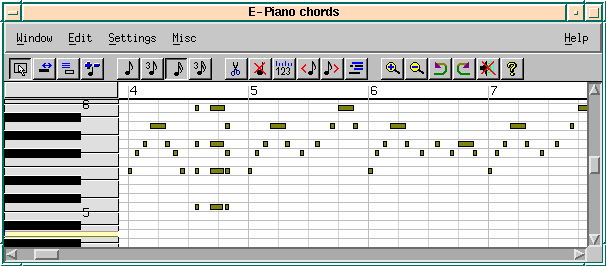
\includegraphics[scale=0.5]{pianowin.png}}
\htmlonly{\image{0cm;0cm}{pianowin.png}}
\caption{Piano Window}
\end{figure}



\section{Toolbar}\label{pwtoolbar}

\begin{figure}
\latexonly{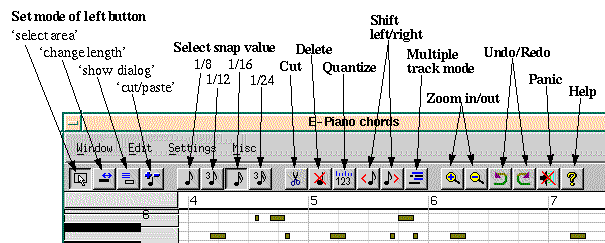
\includegraphics[scale=0.5]{pwtoolb.png}}
\htmlonly{\image{0cm;0cm}{pwtoolb.png}}
\caption{Pianowin toolbar}
\end{figure}

Buttons to set the mode of the left mouse-button:
\begin{itemize}
\item {\em select area} (by dragging a rectangle)
\item {\em change length} (by dragging the 'tail' of an event)
\item {\em show dialog} (\helpref{edit existing event or create a new one}{pweventedit})
\item {\em cut/paste} (great for fast note-by-note editing)
\end{itemize}

Note that these actions can also be done by using other mouse buttons or
by combining shift- and ctrl-keys with mouse buttons
(see \helpref{Mouse actions}{mouseact}).


Buttons to set the most common \helpref{snap}{snap} values (pasted events
will be placed at nearest 'snap' value, similar to a 'grid' in a graphics
paint system):
\begin{itemize}
\item set snap to 1/8 note
\item set snap to 1/12 note
\item set snap to 1/16 note
\item set snap to 1/24 note
\end{itemize}

Buttons to manipulate events:
\begin{itemize}
\item \helpref{Cut}{pwcutpaste}
\item \helpref{Delete}{pwcutpaste}
\item \helpref{Quantize}{quantize}
\item \helpref{Shift left}{pwshift}
\item \helpref{Shift right}{pwshift}
\item Enable {\em multi track mode} as described \helpref{here}{pwevents}
\end{itemize}

Buttons for other operations:
\begin{itemize}
\item \helpref{Undo}{undo}
\item \helpref{Redo}{undo}
\item \helpref{Panic (MIDI reset)}{panic}
\item \helpref{Help}{help}
\end{itemize}



\section{Mouse actions}\label{mouseact}

For a fast reference to mouse-actions, please invoke the {\em Help-$>$Mouse}
menu entry.

{\bf Mouse actions in the event area}

\begin{itemize}

\item {\em Select events}. When in 'select area' mode
(see \helpref{toolbar}{pwtoolbar}), events can
be selected by dragging a rectangle with the left mouse button.
A selection is continued by dragging while holding the shiftkey down. (To
continue a selection outside the current view, you need to scroll using the
window scrollbars before doing shiftkey + left-button again.)

\item {\em Adjust note length by dragging}. Click on the event and drag
the 'tail' while holding mouse button down. This can be done with the
left mouse button when in 'change length' mode
(see \helpref{toolbar}{pwtoolbar}), or by using the right mouse button.

\item {\em Show event dialog}. Opens a dialog box to
modify the values of the event
or to create a new event. This can be done with the left mouse button when in
'show dialog' mode
(see \helpref{toolbar}{pwtoolbar}), or by using ctrl+middle (if
available).

\item {\em Cut / paste events}. Clicking on an event cuts the event to the
internal cut/paste buffer, clicking on an empty position pastes the
buffer contents into the pianowin. This can be done with the left mouse
button when in 'cut/paste' mode
(see \helpref{toolbar}{pwtoolbar}), with the middle mouse button (if
available) or with shift+ctrl+left.

\item {\em Copy events}. Copy an event into the internal cut/paste buffer. Do
this by pressing shift+ctrl+right or shift+middle (if available).

\item {\em Change velocity of event}. Holding the controlkey while pressing the
left or right button on an event increments/decrements the velocity. The
velocity value is displayed in the left end of the top line (just
above the piano keyboard).

\item {\em Change track in 'single track mode'}. You may change the track by pressing
shift + cursor keys.

\item {\em Change track in 'multiple track mode'}. In this mode you can change track
by pressing the right mouse button on an event from another track
(painted with grey color).

\item {\em Listen to pitch}. Do this by pressing shift+right.

\end{itemize}



{\bf Mouse actions in the top line}

\begin{itemize}
\item {\em Start/stop play}. Click the left mouse button on the top line to
start/stop playing (record is not available in the pianowin).
\item {\em Start cycle play}. Select some events (some bars) and press
shift+left-button. If there is no selection active, 4 bars are cycled.
\end{itemize}


\section{Edit/create single events}\label{pweventedit}

\begin{figure}
\latexonly{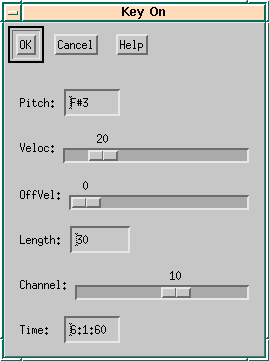
\includegraphics[scale=0.5]{eventdlg.png}}
\htmlonly{\image{0cm;0cm}{eventdlg.png}}
\caption{Example of event editing dialog}
\end{figure}

There are a number of dialogs that allow for detailed editing of single events.
The dialogs are invoked by clicking left mouse button in the pianowin when
in {\em show dialog} mode (see \helpref{toolbar}{pwtoolbar}). Events that
can be created or edited are {\em Note On}, {\em Controller},
{\em Program Change}, {\em Set Tempo} and {\em System Exclusive}.


\section{Edit menu}

Some entries work the same way as discussed in the \helpref{edit menu}{twedit}
of the trackwindow. Only the entries that is special for the pianowindow is
described here.

\subsection{Cut, Copy, Paste}\label{pwcutpaste}
Copies selected events into an internal buffer. Events can be pasted to an
empty space.

Cut is like Copy + delete.

\subsection{Shift}\label{pwshift}

Moves selected events to the left or right. The amount is snaps, which can be
adjusted in the settings-menu.

\subsection{Quantize}
Quantizes selected events to the current snap-setting.

\subsection{Left - Right, Up - Down}

Exchanges the position of selected events. Try it.

\section{Settings menu}

Some entries work the same way as discussed in the
\helpref{settings menu}{twsettings} of the trackwindow.

\subsection{Events}\label{pwevents}

\begin{figure}
\latexonly{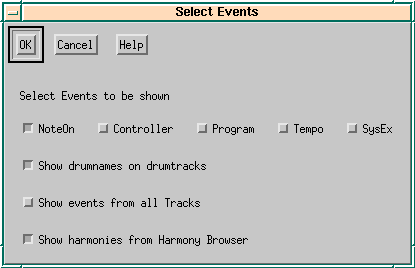
\includegraphics[scale=0.5]{pwevents.png}}
\htmlonly{\image{0cm;0cm}{pwevents.png}}
\caption{Pianowin show-events dialog}
\end{figure}

You can specify what events are to be shown in the pianowin.

\begin{itemize}
\item {\em NoteOn, Controller, Program, Tempo, SysEx}. These events can be
shown and
edited in the pianowin. If you select exactly one, the piano at the left
hand side will be replaced by a list of controller- or program names.
\item {\em Show drumnames}. Switch it off if you prefer to see the piano
keyboard instead of drumnames.
\item {\em Show events from all tracks}. Displays all events
('multi track mode'). Events from active track are shown
red, the others grey. Clicking with the right mouse button on a grey event
changes the actual track.
\item {\em Show harmonies from harmonybrowser}. Displays the chords and
scales from the harmony browser. To see the chords, you must first open the
harmonybrowser and define a chord sequence. Then you have to mark some bars
in the trackwin to show, where the chords should go. Now the pianowin shows
notes from chords in light blue and notes from the scale in light green.

\end{itemize}

\subsection{Snap}\label{snap}

The start time of pasted events will be quantized to this value. This value is also
used in the quantize- and shift dialogs in pianowin and trackwin.


\section{Misc menu}

\subsection{Edit Pitch and others}

\begin{figure}
\latexonly{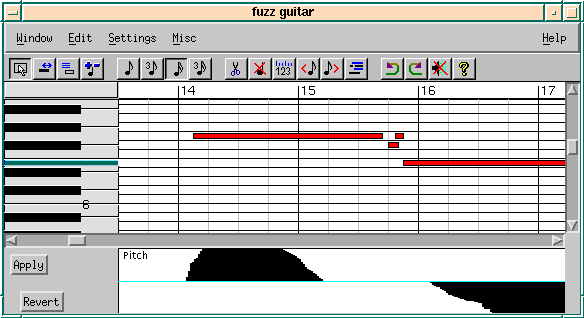
\includegraphics[scale=0.5]{pitched.png}}
\htmlonly{\image{0cm;0cm}{pitched.png}}
\caption{Graphical editing in Pianowin}
\end{figure}


Opens a painting area where you can paint values of the specified type (pitch, controller, ...).
Painting with mouse is done analogous to the \helpref{random rhythm generator}{randrhy}, make sure
you use the right button to set values to zero because you can't paint an exact zero because
of limited screen resolution. Use the Apply button to make your changes take effect.

Also 'tempo' change events can be painted. Please note that tempo changes
in the middle of the song may not work if audio/midi synchronization is
enabled (see \helpref{Global Audio dialog}{globalsettings}).

\subsection{Guitar board}

Opens a window displaying the frets of a guitar. Moving the mouse over the guitar board shows
the names of the notes and moves the black bar in the pianowin. Same works the other way around,
moving the mouse in the pianowin shows the notes on the guitar board.

Also, the actual contents of the pianowin cut / paste buffer is shown (this may be set from the
harmony browser too, so you can see how chords could be played).

Clicking with the left button adds events to the pianowin buffer so you can paste them into
your song. In chord mode (settings dialog), if you add several events to the buffer, they all
start at the same time, otherwise they are generated one after the other (length is the
current snap setting).


\section{Help menu}

\begin{itemize}

\item {\em Pianowin} - loads the pianowin chapter of the help file.

\item {\em Mouse} - displays a dialog that describes mouse actions (what the buttons
do etc.).

\end{itemize}

For more info about help see \helpref{'Help System'}{help} in the {\em Track Window} chapter.

%%%%%%%%%%%%%%%%%%%%%%%%%%%%%%%%%%%%%%%%%%%%%%%%%%%%%%%%%%%%%%%%%%%%%%%%%

\chapter{Audio}\label{audio}

\section{Audio Overview}\label{audiointro}

Audio signal processing is a very CPU and memory intensive task. For
satisfying results we recommend a pentium processor with 32 MB RAM or
up.

The audio part of JAZZ++ is organized similar to a sampler or a
drum machine. That is, you can assign a sound sample to every midi key.
This is different to a usual synthesizer where you assign a sound
to a midi channel and the note only changes the pitch. So an audio track
in JAZZ++ is very much like a drum track. On a drum track, every
note plays another instrument, on an audio track every note plays
another sample.

You assign samples to midi keys using the \helpref{Sample Settings
Dialog}{samplesettings}. JAZZ++ then loads the samples into memory. You
may use samples with different sampling rates and channels (mono,
stereo) in one song, JAZZ++ converts all samples into the format you
specify in the \helpref{Global Settings Dialog}{globalsettings}.
The collection of samples you define in the Sample Settings Dialog
is called a {\em Sample Set} in JAZZ++.

After defining a sample set, you should define an audio track. You do
this in the track window by opening the \helpref{Track Dialog}{trackdlg}
and check the entry called Audio Track. Audio tracks behave the same
way like drum tracks or other midi tracks. E.g you can place individual
notes on the track, copy, delete or replicate bars etc. Every note
on the audio track corresponds to a sample you just defined.

\begin{figure}
\latexonly{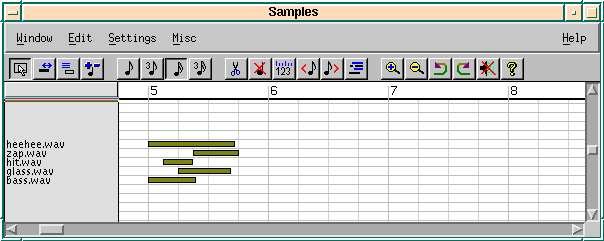
\includegraphics[scale=0.5]{audiotrk.png}}
\htmlonly{\image{0cm;0cm}{audiotrk.png}}
\caption{Audio track in pianowin}
\end{figure}

Next open the piano window on that track by clicking with the right
mouse button on the audio track you just created. When you scroll up
and down you should see the labels of the samples on the left hand side
of the window (the labels are assigned in the Sample Settings Dialog).
When you click on one of the labels, you should hear the sound of
that sample.

Next select the 1/16 note in the toolbar to be able to place some notes
on the track. Then set a few notes. When placing a note, you will hear
the sample too. Also you may notice, that the length of the note is
not 1/16 but is as long as the sample is according to the current midi
speed. When you change the midi speed in the trackwin, you will see that
the note length is adjusted to the new speed (by the way: this way you
can easily adjust the midi speed to a drum loop sample).

Now you are ready to listen to your new song. Go back to the track
window and click on the start play toolbar button. And voila, you will
hear your new audio enabled song.


\section{Audio Recording}

Audio record works much the same way like midi record. Select some bars
on an audio track where you want to record an audio signal. Then press
the record button. More on record / play you can read
\helpref{here}{recplay}.  While recording you may not hear other samples
depending on the capabilities of your sound card. Most sound cards do not
support simultaneous record and playback.

When you have finished recording, stop the operation by clicking on the
play or record button again. JAZZ++ will then ask you, if you want to
keep the recording.  When you answer yes, you will get the file selector
dialog to specify the audio file for your recording. The recording will
be saved in the Microsoft .wav format.  Also JAZZ++ automatically assigns
a midi note to your new sample and places a note on the recorded audio
track.  If you don't like your recording and you do it again, you should
save it under the same file name as the old recording. Then JAZZ++ will
reuse the same midi note and not assign a new one.

Please note: when you do audio recording, JAZZ++ needs much memory for the
playback too. So you should start playback a few bars before the
selection and stop playback a few bars after it. Please do not playback
the whole song, when you only want to record a few bars.


\section{Audio Menu}

\subsection{Global Settings}\label{globalsettings}

\begin{figure}
\latexonly{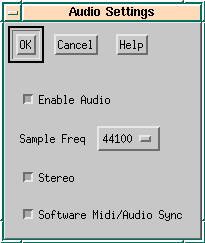
\includegraphics[scale=0.5]{audioset.png}}
\htmlonly{\image{0cm;0cm}{audioset.png}}
\caption{Global audio settings dialog}
\end{figure}

Here you specify the internal resolution for the audio processing of
JAZZ++.  This means, that all samples are internally converted to the
parameters you specify here. If you set the sampling rate to 22050 here
and load a sample that was sampled with 11025 samples per second, JAZZ++
will convert it to 22050 samples per second on loading. Specifying
low quality here (low sampling rate and mono) will dramatically reduce
the CPU and memory requirements needed for processing. Of course this
will reduce sound quality too.

\begin{itemize}

\item {\em Enable Audio}. If you leave this unchecked, the whole audio system
will be disabled. This is useful, if you do not use audio in a midi-only
song and want to save CPU and memory.

\item {\em Sample Freq (or Sampling Rate)}. The number of samples per second and
per channel (if stereo). 44100 is CD quality, 8000 is telephone sound.

\item {\em Stereo}. Switch this off if all your samples are mono anyway or to
save memory.

\item {\em Software Midi/Audio Sync}. You may try to switch this off. If midi
and audio keep in time, then your sound card synchronizes midi and audio
itself and you should leave this unchecked, because midi-audio synchronization
is CPU intensive too. Most cards do not synchronize midi and audio, so
in most cases this should be checked. Please note that midi tempo changes
in the middle of a song will not work if Midi/Audio Sync is enabled.

\end{itemize}



\subsection{Sample Settings}\label{samplesettings}

\begin{figure}
\latexonly{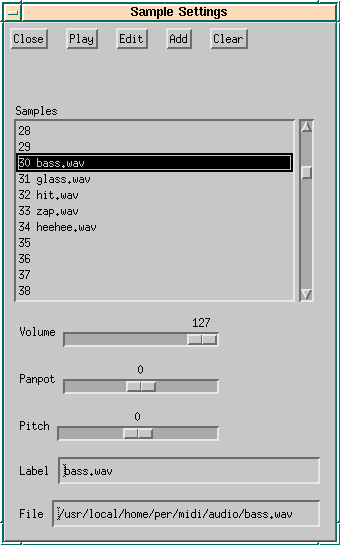
\includegraphics[scale=0.5]{sampset.png}}
\htmlonly{\image{0cm;0cm}{sampset.png}}
\caption{Sample settings dialog}
\end{figure}

In this dialog you define the midi keys for your samples. Please read
the \helpref{Introduction}{audiointro} for more information on midi
keys for samples.

You add a new sample to the list by selecting an list entry first
and then press the add button. In the file selector you choose the
sample file you want to play in your song. The only file format supported
currently is the Microsoft .wav format. After loading the file you should
enter a label (a name for the sample) in the label text entry near the
bottom. This label will be shown in the piano window when editing an
audio track.

The list shows the available midi keys at the left. Low numbers at the
top of the list stand for very low midi keys and high numbers for high
midi keys. To avoid scrolling in the piano window you probably want to
load the samples somewhere in the middle of the list.

To remove a sample from the list select that entry and press the Clear
button. To listen to a sample press the Play button, to interrupt
listening press it again. The Edit button invokes the \helpref{Sample
Editor}{samplewin}.

The Sample Settings dialogs also allows to adjust volume, pan and pitch
of a sample. In opposite to the Sample Editor, these changes are not
permanent, e.g if you reduce the volume you can increase it later again
with no loss of quality. JAZZ++ applies these settings every time a sample
is loaded.

After you have defined a set of samples you want to use, you may
save these settings into a .spl file. Close the dialog and select Save Set from the
Audio menu in the track window. Please notice, that these files contain all
your settings from the Sample Settings Dialog, but they do not contain
the samples themselves. The .spl files only contains the filenames of
the samples, so if you rename or delete samples, JAZZ++ will not be able
to find those samples again.

\section{Sample Editor}\label{samplewin}

\begin{figure}
\latexonly{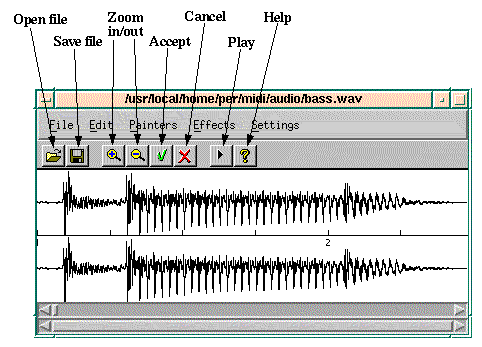
\includegraphics[scale=0.5]{sampedit.png}}
\htmlonly{\image{0cm;0cm}{sampedit.png}}
\caption{Sample editor}
\end{figure}

The sample editor may be invoked from the
\helpref{Sample Settings Dialog}{samplesettings} or from the piano window.
In the piano window, the editor is invoked when you select the dialog
toolbar button on an audio track and click on a note.

The sample editor shows the waveform of the audio signal and allows
you to modify it. There are two scrollbars, the upper one controls the
zoom and the lower one the view position.

For some operations (like cut) you must select a range of samples, you
can do this by dragging the mouse. Similar to the track window or piano
window you may continue a selection by dragging with the shift key down.
Clicking again clears the selection. Other operations (like paste) need
an insertion point. This is set by clicking into the sample area when
there is no selection. The insertion point is displayed as a vertical
red line.

A more convenient way to zoom into a part of a sample is to select
the range of interest and then click the magnify glass button.

Pressing the play button will play the whole sample by default. If there
is a selection, only the selected samples will played. If there is
an insertion point, play will start at that point.



\subsection{Loading and Saving Samples}

After you have modified your sample you may save it. Please note that
saving will make the settings in the \helpref{Sample Settings
Dialog}{samplesettings} permanent. That is, if you have set the volume
e.g. to a value of 50 in the sample settings dialog, the sample will be
saved with this volume and you cannot make it louder again without loss
of quality. To avoid this, you can set the volume to maximum in the
sample settings dialog and leave the pan and pitch sliders neutral before
starting to edit. After saving your sample you can change volume etc again.

You may think of the sample settings dialog as some kind of mixer
whereas the sample editor really changes the sound source itself.

\subsection{Cut/Copy/Paste}

\begin{itemize}

\item {\em Cut}. Cuts out a piece of the sample into an internal buffer. Needs
some samples to be selected.

\item {\em Copy}. Copies some samples into the internal buffer. If no range is
selected, the whole sample is copied.

\item {\em Paste}. Inserts the samples from the internal buffer to the sample.
If there is a selection, the selection is replaced by the buffer. If there
is an insertion point, the buffer is inserted at that position.

\item {\em Paste Merge}. Adds the buffer at the insertion point. The samples
from the buffer are mixed with the original.

\end{itemize}



\subsection{Silence}

You have to select a range before using this function.
\begin{itemize}
\item {\em Replace} - the selection will be replaced with silence.
\item {\em Insert} - will insert silence at the beginning of the selection,
the length of the inserted silence is equal to the length of the selection.
\item {\em Append} - will append silence at the end of the selection. The
length is equal to the length of the selection.
\end{itemize}


\subsection{Invert Phase}
Inverts the phase of the left or right channel


\subsection{Maximize Volume}
This maximizes the volume of the whole sample. It is made as loud as possible
without distortion.


\subsection{Painters}\label{audiopainters}

After selecting a painter command in the menu bar, a paintable area is
displayed at the bottom of the window. In this area you may paint some
kind of curve. Painting works the same way as in the \helpref{Random
Rhythm Generator}{randrhy} and is described there in more detail. After
painting you can press the green accept-button in the toolbar or the red
crossed cancel button. The operation is applied for the visible range
of samples. So if you don't want to modify the whole sample, zoom to
the range of interest before invoking the painter.

\begin{itemize}
\item {\em Volume} - lets you paint some kind of envelope. The painter lets you
paint the relative volume, that means no painting will not change the
volume, painting above the zero line will increase the volume, painting
below the zero line will decrease it.
\item {\em Panpot} - changes volume between left and right channel
\item {\em Pitch} - changes the pitch of the sample. This can operate on the
whole sample only. The range of transposing can be adjusted in the
Settings menu.
\item {\em Filter} - a dynamic filter, e.g you can paint the cut off frequency.
The filter settings can be adjusted in the settings menu.
\end{itemize}

% how to use, Pitch Painter Settings
% volume pan pitch filter


\subsection{Distortion}

This adds a distortion effect to your sample. In the dialog you can paint
a distortion curve. When pressing Ok, every sample is mapped to a new
value according to the curve. JAZZ++ looks up the original sample value at the
horizontal axis and replaces the sample value with the height value of
the curve at that point. Because painting smooth curves is difficult, there
are some presets, try them out!



\subsection{Reverb}

The reverb algorithm of JAZZ++ is produces a high quality reverb effect.
Parameters of the Reverb Dialog:

\begin{itemize}
\item {\em Room Size} - a value corresponding to the time until the first
echo of the reverb can be heard. If you think of a big room producing
the reverb, this corresponds to the size of the room.
\item {\em Brightness} - controls the frequencies that are echoed from
the rooms walls.
\item {\em Length} - controls how many echos are computed. This controls the
depth of the reverb.
\item {\em Effect Volume} - the final output mixer, you set the volume of the
reverb-only signal here which is mixed to the original then.
\end{itemize}



\subsection{Echo}

In this dialog you can add one or more echos to your sample.
\begin{itemize}
\item {\em Number of echos} - controls how many echos are generated
\item {\em Delay} - the time in milli seconds between the echos
\item {\em Amplitude} - the relative Amplitude in \%. A value of e.g. 20 means,
that the first echo has a volume of 20\% of the original, the second
echo has a volume of 20\% of the first echo and so on.
\item {\em Random delay}. If this is checked, the time between the echos is
chosen randomly. The Delay-Value (see above) is taken as a basis
for the random generator.
\end{itemize}




\subsection{Chorus}

This is some kind of universal effect which can produce chorus-like effects.
The operation is quite simple: JAZZ++ takes a copy of the original sample,
then modifies it according to the settings in the dialog and finally
mixes the modified copy back to the original.

\begin{itemize}

\item {\em Delay} - delays the signal for the number of seconds/100 specified
here (e.g. a value of 20 means 200 millisec delay).

\item {\em Pitch Modulation Frequency} - changes the pitch of the signal up
and down controlled by a sine wave LFO (Low Frequency Oscillator), this is
the heart of most chorus effects.
The modulation frequency is set in Hertz/10 (that is, a value of 20 means 2
turnarounds per second). The modulation frequency corresponds to the speed
regulator of a chorus effect.

\item {\em Pitch Intensity} - the depth of pitch change.

\item {\em Pan Freq} - changes the pan of the signal to the left and right
controlled by a sine LFO.

\item {\em Stereo Spread} - enhances the stereo effect of the output. You
may even try to convert a mono signal to a stereo signal by setting Delay
to 20 or so, turn pitch intensity and pan spread off and set stereo spread
to maximum.

\item {\em Effect Volume} - the volume of the modified signal in \% of the
original.

\end{itemize}



\subsection{Pitch shifter}\label{pitchshifter}

This operation lets you change the pitch of a sample. Pitch changing
normally changes the length of the sample too (you can think of a tape
machine, where the speed is altered). JAZZ++ however provides algorithms
to change the speed without changing the length of the sample.

With the sliders you specify the amount of transposition in semitones.
If the box {\em Keep Length} is checked, the transposed sample will have the
same length as the original. In this case, JAZZ++ divides the sample
into small pieces and plays these pieces with the new speed as often as
necessary to match the original length. This may lead to an undesired
tremolo effect if the size of the pieces is too big or too small. The
slider named window size lets you adjust the size of the pieces.


\subsection{Time Stretcher}

This is similar to the \helpref{Pitch shifter}{pitchshifter}. You can
change the length of the sample here. Changing the length normally
changes the pitch of the sample too, but if you check the box labeled
{\em Keep Pitch} JAZZ++ will change the length without changing the pitch.

You may specify the new length in seconds (upper sliders) or in terms
of midi speed (lower sliders). With the upper sliders you specify the
delta length, that is how much time you like to add or subtract from
the original length. Eg to make the sample one second shorter, you
would set the first slider to -1.

The midi speed sliders are best explained using an example: Lets assume
you have a drum loop recorded at a speed of 120 beats per minute. To
change the speed (and thus the length) of the sample, to 130 beats per
minute, you set the slider {\em old speed} to 120 and the slider {\em new speed}
to 130.

The meaning of the window slider is described in the \helpref{Pitch
Shifter Dialog}{pitchshifter}.



\subsection{Reverse}

This reverses the output (think of a tape playing backwards). If there
is no selection, the whole sample is reversed.



\subsection{Additive Synthesis}

In this window you can generate new sounds using a noise generator
together with additive sound synthesis generators. You may up to 6
generators to build your sound. For each generator you can paint curves
for envelope, panpot and pitch. The output of all generators is mixed
together to make the final sound.

The toolbar buttons have the following meaning (from left to right):
\begin{itemize}
\item load synth settings. In the song subdirectory you find an
example for a simple drum which maybe a starting point for you.
\item save a synth settings.
\item generate a wave
\item listen to the generated wave (you have to generate first). If you
don't hear anything make sure that you have painted some envelope. Also
you have to enable audio in the audio menu of the track window of course.
\end{itemize}

Near the top of the window you find some checkboxes. The first
4 (Harmonics, Envelope, Panpot and Pitch) switch on and off the
corresponding paint areas.  This is useful for painting on a small screen.
The last one labeled {\it Noise} turns the first generator into a noise
generator when checked.

{\bf Noise generator}

In the left paint area labeled {\it noise filter}  you can paint the
cut off frequency of the noise generator. The slider labeled {\it Midi Key}
is ignored in the noise mode.


{\bf Sound generator}

In sound generator mode the left paint area is labeled {\it harmonics}. You can
paint the volumes for each harmonic. Note that the 10 leftmost harmonics
determine much of the final sound (you have to make the window big to
paint these). Harmonics with even numbers sound warmer than harmonics
with odd numbers. Most sounds will only have a few harmonics with
high volume and especially harmonics with high numbers will have low
volume. In this mode the midi key is the base frequency from which the
harmonics are calculated.

{\bf working with multiple generators}

With the slider labeled {\it Number of Synths} you can use up to 6 generators
simultaneously. Only the first one may be a noise generator, all others will
be in additive synthesis mode. There is much room for experimenting with
multiple generators, e.g you can do some kind of morphing / cross-fading with
the envelope painters, or get some chorus like effects when detuning the
oscillators a little bit in the pitch painter.

After you have made some sound make sure to add some reverb or chorus.



\subsection{Filter}

This adds high quality filters to your effects gallery. You may choose
one of the following filter types:

\begin{itemize}
\item {\em Low Pass} - lets pass low frequencies, the volume of high
frequencies is reduced (some kind of bass booster).
Frequencies below the corner frequency will become louder, frequencies above
will become more quiet. The bandwidth value is ignored.

\item {\em High Pass} - the other way round, the volume of low frequencies is
reduced and high frequencies can pass the filter (some kind of treble booster).
Frequencies above the corner frequency will become louder, frequencies below
will become more quiet. The bandwidth value is ignored.

\item {\em Band Pass} - increases the volume of middle frequencies. The corner
frequency is the frequency with maximum volume. The bandwidth is a value
in \% of the corner frequency and specifies, what frequencies above
and below the corner frequency may pass the filter.

\item {\em Band Stop} - decreases the volume of middle frequencies.
\end{itemize}

The feedback value controls the gradient of the filter. In case of a low
pass filter for example, it controls how much the volume above the
corner frequency is reduced. A value of 1 or 2 is sufficient in most
cases.

\subsection{Settings}

\begin{itemize}

\item {\em Pitch Painter} opens a dialog to control the range of the
pitch paint area (see \helpref{Painters}{audiopainters}).

\item {\em Filter Painter} opens a dialog to control the type of filter that
is applied to the filter painter area (see \helpref{Painters}{audiopainters}).

\item {\em View Settings} opens a dialog to control view parameters of the
sample editor window. The 'show midi time' checkbox toggles between
showing time as counts or real time.

\end{itemize}

%%%%%%%%%%%%%%%%%%%%%%%%%%%%%%%%%%%%%%%%%%%%%%%%%%%%%%%%%%%%%%%%%%%%%%%%%

\chapter{Examples}\label{examples}

\section{How to build a new midi song}\label{exmidisong}

Supposing you start with a blank song in the trackwin, these are the steps
you need to do in order to record some midi tracks and make your own midi song.

\begin{enumerate}

\item {\em Turn on the metronome}. Push the \helpref{metronome button}{twtoolbar}.
This will help you keep in time when playing.
Later, when you have recorded some tracks, you may want to turn the metronome
off again because the other recorded tracks will support you with the necessary
beat information.

\item {\em Select counts per bar etc.}. By default, a blank song will have
4 counts per bar with each count corresponding to a quarter note. To change
this you need to invoke the \helpref{Misc-$>$Meterchange}{meterchange}
menu entry.

\item {\em Select song speed}. You probably have a feeling about how fast
your song should be. You can try this right away by just pressing the
\helpref{play button}{twtoolbar}. You will then hear the beats of the
metronome. Change the speed to your preference by clicking into the
\helpref{speed field}{speed}.

\item {\em Define track defaults}\label{rectrackdef}. Before you can enter music
(events) into
a track, you need to define {\em track name}, {\em instrument to be played}
and {\em midi channel number} for that track. Do this by clicking on the
\helpref{track name field}{trackdlg}, starting on the {\em second} track (will
invoke the Track Settings dialog). {\em Never use the first track for
recording}, as this is defined to be the {\em master track} (holding events
controlling the whole song like speed, meter change etc.).

\begin{itemize}

\item {\em Track name}. Enter a track-name that describes what you play on the
track, not just the instrument
name (you may want to play some other voice using the same instrument into
another track at a later stage).

\item {\em Instrument}. Select an instrument from the instrument list. The instruments with
one number in front of the name (e.g. '5 Rhodes Piano') are the 'General MIDI' (GM)
instruments, the others are extensions to the GM standard and may not be
supported by your synth/sound-card.

If this track is to play the same
channel and the same instrument as a previously defined track, set the
instrument to 'None' (default).

If your track is a drum track, the instrument names are a bit misleading.
To get started we recommend that you select instrument number 1
(labeled '1 Piano 1'). This will give you the 'standard drum kit' on a
GM compatible synth/sound-card. You must study the instrument list in your
synth documentation to see what other drumkits are available.

\item {\em MIDI channel}. If the track is to play a new instrument, choose a
midi channel that
has not been used by another track. Start at channel 1 and increment by one
for each new instrument (track). If your track is to play {\em drums}, select
channel 10 (predefined by GM to be the drum channel).

\end{itemize}

\item {\em Set output midi channel on your keyboard}\label{recsetkbchan}.
If your keyboard is
capable of sending on different midi channels, you should now set the
keyboard output channel according to the midi channel of the track you are
about to record. If your keyboard can only send on one midi channel
(e.g. channel 1), you must use a slightly different algorithm
(described \helpref{below}{onechannel}).

Note that you can also 'record' without a keyboard by manually entering
events into the \helpref{pianowin}{pianowin} using the mouse.

\item {\em Select some bars}. \helpref{Select}{select} the area of your track
where you want to record. You can also select the whole track by
clicking in the leftmost field of the track in trackwin (the
\helpref{track/channel display column}{trackdefs}).

\item {\em Start recording}. Start recording by clicking at the
\helpref{record button}{twtoolbar}. JAZZ++ will then start to play one bar
ahead of the selected area to give you a count-in. You can also start
recording by clicking directly at a bar in the top-line of the event area
(see section \helpref{Record and play}{recplay}). While recording you will
hear the metronome (if enabled), any previously recorded tracks plus your own
keyboard playing.

\item {\em Stop recording}. Stop recording by clicking the
\helpref{record button}{twtoolbar} again (or use one of the other 'stop-play'
methods). If you played any notes, you will be asked if you want
to keep the recorded events. If you decide to keep them, press 'Ok'. You can
then listen to the recording. If you are not satisfied you can press the
\helpref{Undo button}{twtoolbar} to take it away and then do a new recording
(go back to previous item).
You can also do a new recording by pressing right-button on the top-line.
The old recording will then be silent, and any new recording will replace the
old one.

\item {\em Post process the recording}. You may want to fix something in your
recording afterwards. You may want to \helpref{quantize}{quantize} or
\helpref{transpose}{transpose} the recording (menu entry {\em Edit-$>$Transpose}),
or you may want to fix notes that are wrong using the mouse in the
\helpref{pianowin}{pianowin}.

\end{enumerate}

You can record a new track by going back to the item
{\em 'Define track defaults'}. You can also record more
music into an existing track by going back to item
{\em 'Set output midi channel on your keyboard'}.

At some point you will probably also want to edit other track defaults like
volume, pan, reverb and chorus. You can do this by invoking the
\helpref{Mixer}{mixer} dialog (press the \helpref{mixer button}{twtoolbar}).

If your synth is {\em GS} or {\em XG} compatible, you may also want to do other kinds of
part editing like adjusting {\em sound-color}, {\em vibrato} or {\em envelope},
or change the behavior of controllers like {\em pitch bender} and
{\em modulation wheel}. These things and a lot more are accessible through the
\helpref{Parts menu}{partsmenu}.

\subsection{Recording with a one-channel keyboard}\label{onechannel}

If your keyboard can only send on one midi channel (e.g. channel 1) you must
change the above procedure according to the following:

\begin{itemize}

\item Always record in a track having the default channel set to 1.

\item When finished recording on that track, change the default track number
to something else (a free channel number) by clicking the track-name-field
and adjusting the slider in the "Track Settings" dialog. When you click
'Ok', the default channel and all events on the track will be converted to
the new channel number (this is true if the entry
{\em 'Force channel number onto all events on track'} is checked).

\item If you want to do more recording on a previously recorded track, change
that track back to channel 1 first using the same method.

\end{itemize}

Pressing the \helpref{Panic}{twtoolbar} button between operations will
prevent the synth/sound-card from being confused (sends a 'reset' command
to the synth/sound-card).


\section{Random rhythm and harmonizer example}

This section documents the demo example.

\begin{enumerate}

\item I prepared the tracks for the song and assigned names and channels for
drums, bass, piano and melody. Then I generated the drums with the
random rhythm generator.

\item open the random rhythm generator and load the file demo.rhy. Lets take a
look at the adjustments for the instruments:

The first kick drum defines high probabilities at beat 1/4 and 3/4 -
this makes the basic groove. The probabilities at 3/16 and 9/16 are a
little lower, so the kick drum will not play these beats always. The
velocity ranges from about 70 to 100, so the loudness of the beats varies.

The snare drum plays at 2/4 and 4/4 but probabilities are less than 100\%, so
it will play most of the time but not always. The velocity is about 80 .. 100, so
the snare is loud always, there is not much dynamic.

The third entry, closed hi-hat, plays at 2/8, 4/8, 6/8 and 8/8 - the probabilities
are 100\% and velocity is high - these beats are played always and all of them are
loud.

The ride cymbal plays most of 1/4, 2/4, 3/4 and 4/4 and sometimes on 16/16. Also
it plays at 9/16 - just to make things more interesting.

The next entry, snare drum again, plays with low probability on all 1/16 timings -
so not all of them are played - the probabilities would lead to about every 2nd
1/16 would be played. For every beat that is played, the generator selects a
length from the length field. Valid length values are 1/16, 2/16 and 3/16 where
1/16 is chosen most often because it has the highest probability. When a length
greater 1 is selected, then the generator will not produce a beat on the following
1/16 step, because the previous note has not finished. Anyway, the velocity is
very low compared to the other snare drum entry. Together both snare drum entries
produce a loud and steady beat from the first entry and a lot of low-velocity
fillings from the second entry.

The last entry, closed hi-hat again, is similar. It does not play on the timing positions
where the first closed hi-hat plays its loud and steady beats. It plays at the other
timing position in between with a very wide range of velocity - so some of these
in between beats will be dominant while others will sound like background.


\item To produce the rhythm I selected bar 5 to 20 on the drum track and then
clicked on the 'gen' button. This gives demo1.mid

\item next I recorded 2 bars of a bass line and some chords. I quantized
this and set the velocity to 90. Last I choose repeat copy to duplicate
the material to the full length of 16 bars. This is demo2.mid.

\item next I recorded a melody and did some corrections in the pianowin editor.
This is demo3.mid.

\item last I wanted some more interesting harmonies. To reproduce this step
you may open the harmony browser and load the file demo.har.

The first 4 chords
are from the original recording Am7 and D7. These are step II and V from G major.
So I chose Gj7 as the next 2 chords to establish that scale.

The next 6 chords are a minor II-V-I move, which leads to Bbm7 in the
scale of Ab major - notice, that the V was taken from the harmonic scale.
The last chords are a V-I move in Ab major.


\item to perform the transposition, transpose every track on its own. Mark the
bass track in the trackwin and select transpose in the harmony browser (the button
where the arrow points from the rectangle to the note). Then do the same for
piano and melody. This should result in demo4.mid.

demo4.mid is not perfectly transposed, but it could serve as a starting point and
you could correct some notes in the pianowin editor. The pianowin editor can
show the chords and scales in colors, look at \helpref{Pianowin Menu Events}{pwevents}
for details.

\end{enumerate}


\section{Audio example}\label{exaudio}

This is how you run the supplied audio demo:

\begin{enumerate}

\item Load the midi file named 'audiodem.mid'. You will see there are 3 tracks
defined; drums, bass and an audio track named 'guitar'.

\item Invoke menu entry {\em Audio$->$Load Set} and load file 'audiodem.spl'.
This is the 'sample set definition file' that binds audio sample files to
the different key pitches (see \helpref{Audio Overview}{audiointro}).

\item Check that audio is enabled (invoke menu entry
{\em Audio$->$Global Settings}, see \helpref{Global Settings}{globalsettings}).

\item Now you can play the song (with audio) (see
\helpref{Record and Play}{recplay}).

\end{enumerate}

You may also want to look at how the samples are bound to the key pitches by
invoking
\helpref{Sample Settings dialog}{samplesettings} and scroll the listbox down to
position 50. There are two samples defined (funkguit1.wav and funkguit2.wav).
Play the samples by selecting in the listbox and press the {\em Play} button.
Look at how you can edit the samples in the
\helpref{Sample Editor}{samplewin} by pressing the {\em Edit} button.

At last you should look at the 'guitar' audio track in the
\helpref{Piano Window}{pianowin}. Scroll
up and down until you find the defined samples.



\chapter{Appendix}\label{appendix}
The appendix has not been appended yet, come back soon!

\chapter{RoadMap}

\section{Frequently Asked Questions}\title{FAQ}

\section{Jazz++ Specific}

\section{How powerful does my computer need to be to run JAZZ++ properly?}


It is best to understand here, that it's not so much a matter of how much raw
processing power your computer has -- it's more to do with JAZZ++ and other
MIDI softwares being able to do what they want to do, -exactly when- they want
to do it. If another software process happens to be using the CPU and OS at the
exact same moment JAZZ++ or another MIDI program wants to send a MIDI event or
else send PCM data to the soundcard (and both these things have to happen
almost simultaneously), one or another process is going to have to wait. That
can't technically happen in the MIDI domain, because the real time nature of
compositional recording and playing doesn't allow for such.

In practise, there's a tiny 'window' in time for MIDI to complete any note
event cycle. The practical size of this 'window' is roughly bounded by the
average human ear perception of what is actually 'in sync' and what is 'out of
sync'. This percepton 'window' tends to vary from individual to individual,
but for example only here, most people don't perceive things being 'out of
sync' during MIDI performances, provided the note event 'window' isn't longer
than 20 milliseconds or so. However, in the case of music, it's perhaps better
not to play the note at all, if it's too far out of time with the composition,
and that 'window' definitely closes when it comes time for the next MIDI event
on the same channel or track. If your MIDI note event or softsynth is put on
wait trying to access the CPU and hardware, this 'window' becomes even smaller.

If you use JAZZ++ with MIDI software synths and drum-machines etc, all these
processes compete against each other for a slice of CPU time. Critically, they
will all want to do this at exactly the same time in empathy with the real time
nature of the MIDI compositional playing or recording processes. At a hardware
level, this is sometimes impossible to do. This is especially so when you've
got MIDI softsynths running. Consider the analogy of a MIDI softsynth program
as being akin to the old original analog synthesizers that used many discrete
electronic components and circuits to create the actual sound one hears. Unlike
these real world hardwares however, where one merely applies power and the
hardware does the rest with sound emerging at end, MIDI softsynths require CPU
cycles to render the waveform data and pass that onto the soundcard itself, to
recreate the sound that you will eventually hear.

This being the case, imagine you're replaying a MIDI composition using JAZZ++
and a softsynth, to recreate the sound of a traditional string quartet. During
replay, three of the instrument voices are engaged in a harmonic drone, while
the lead violin plays solo.... 

[ed: TBC.. ]

\section{Windows Specific}

[ed: TBC.. ]

\section{Linux Specific}

Here you will find topical reference for using JAZZ++ with Linux

Note: At this time the following is only tested and known to be true when using
JAZZ++ with Linux on Intel based ix86 architectures in both 32 and 64 bit
flavors. If you are using Linux on another hardware platform, the following
should be treated as a guide only. 

Q. Does Jazz++ work on all Linux distributions?

A. Jazz++ should work on most all current Linux distributions. If there are
no binary packages available to suit your particular installation, Jazz++
should build, install, and run currectly from the source code contained in
either the release tarball or the Jazz++ svn repository. Note: The source 
code obtained from the Jazz++ svn repository should be considered as being
the 'unstable' development branch of the Jazz++ tree. Some Linux users may
find that they have to update their system kernel (see below), however if
you don't wish to (or don't feel up to) changing the Linux kernel on your
installation, you might consider the following ;

  "It seems some Linux distibutors are now moving towards multimedia and
  audio-visual 'studio' type sub-distributions, specifically aimed for
  people wanting to use Linux in this area. These distribution releases
  have the low-latency, so called 'real time' (RT) Linux kernel build as
  standard, and this can 'ease the pain' for a lot of Linux users..."

  
Q. Do I need a low-latency or 'RT' Linux kernel to run Jazz++ ?

A. The answer to this question largely depends on what sort of Jazz++
user you might be...ie; 'casual' or 'serious'....and exactly what kind
of (MIDI) hardware you are using to render the actual sound with...ie;
hardware MIDI/synth or softsynth. Generally speaking, if you experience
latency problems with either the MIDI transports and/or sound rendering
using softsynths, it is very likely you will need a 'RT' Linux kernel.
Such latency problems can manifest themselves in a number of ways. (see below)


Q. What are 'latency problems' when using Jazz++ with Linux?

A. There are a couple places Linux kernel latency issues will obviate
themselves. Each is a little different from the other, and one or more of these
things might happen at any same given time -- they share a common cause.

    1. When using Jazz++ on Linux with externally connected MIDI equipment
    and/or hardware MIDI/synth soundcard, your computer is only dealing with
    the MIDI data being orchestrated by Jazz++. It can happen, especially
    during complex MIDI passages, that certain notes are being seemingly
    'dropped' on one or more channels. 

    2. When using Jazz++ on Linux with software MIDI synthesizers, your
    computer has to deal with transporting the MIDI data *and* render the
    actual sound your hear as well. In this case, not only might there be
    'dropped' notes, but also the actual sound of the softsynth might be
    distorted, or have other unwanted sound artifacts such as 'clicks' or a
    harsh scratching noise - it varies on the type of softsynth used and
    just how bad the actual problem itself is.

Remember, Jazz++ itself is only dealing with MIDI data (when not being
used cojointly with the audio mode features), and it attempts to both
generate and receive that MIDI data in as close to real time as possible.
However, getting this MIDI data to/from Jazz++ itself and real MIDI hardware
devices, necessitates real time access to the actual -computer- hardware
itself, and the -only- way that can happen is via the running Linux kernel.

Likewise, softsynths have to actually render the sound data, and have real time
access to the soundcard (PCM) ports, and this too has to travel through the
Linux kernel layer. The only solution is to change your Linux kernel if you
come across problems like these using Jazz++ on Linux, and in fact you might
have to do this anyway if you intend to use a MIDI softsynth.


Q. I think I have the above problems, where can I get a 'RT' Linux kernel?

A. With some 250+ Linux distributions out there, this will never be an
exhaustive list -- however, here are some pointers to help people out ;

    1. Definitive: The latest Linux kernel release is always available from
    www.kernel.org and mirrors. At the time of this writing, the 'current'
    stable Linux kernel is the 2.6.25.4 release. If you're up to configuring
    and installing the Linux kernel from source, currently the 'RT' patches
    are available at www.kernel.org/pub/linux/kernel/projects/rt/  

    2. I found this on a webpage: - "Many distributions have at least one 
    specialised low-latency kernel package available via some sort of 
    additional multimedia distribution or repository; consider using one of 
    these. For example, Ubuntu -> Ubuntu Studio; Debian  -> 64 Studio or Musix;
    Fedora  -> PlanetCCRMA; OpenSUSE -> JAD."

    3. Ubuntu: (quote) "Lowlatency kernel is in standard ubuntu repositories,
    just run: 

    sudo apt-get install linux-lowlatency

    Then reboot and select that kernel from the GRUB list. It should have no 
    detrimental effects at all on normal usage."

    4. Debian: Have a look here ;

    http://apt.64studio.com/64studio/testing/pool/main/l/linux-2.6/

    Although these are intended for the 64studio release, these packages
    may work with the current Debian 4.0 branch. There are also 32bit
    packages here as well.

    5. Mandriva: Have a look here ;

    http://wiki.mandriva.com/en/Docs/Howto/Mandriva\_Kernels\#kernel-rt

    6. Fedora: Have a look here ;

    http://ccrma.stanford.edu/planetccrma/software/installplaneteight.html

    7. Other linux distributions: Yours not listed? Perhaps you know how
    to address this issue with the Linux distribution you are using, and
    would like to tell us? See the Jazz++ MailingList and let us know?

Q. When I start jackd/QJACKCTL I get the following error, what's wrong?


\subsection{Other MIDI software known to work with JAZZ++ and Linux}

The following may never be a complete list of MIDI software synthesizers and
other MIDI based programs that work with JAZZ++ and Linux today, however we take
the time here to mention some of the more popular and actively supported
softwares of this type, that members of the JAZZ++ team have tried and tested.

[ed: TBC.. ]


\section{Mac Specific}

[ed: TBC.. ]

\end{document}
